%%%%%%%%%%%%%%%%%%%%%%%%%%%%%%%%%%%%%%%%%%%%%%%%%%%%%%%%%%%%%%%%%%%%%%
% How to use writeLaTeX: 
%
% You edit the source code here on the left, and the preview on the
% right shows you the result within a few seconds.
%
% Bookmark this page and share the URL with your co-authors. They can
% edit at the same time!
%
% You can upload figures, bibliographies, custom classes and
% styles using the files menu.
%
%%%%%%%%%%%%%%%%%%%%%%%%%%%%%%%%%%%%%%%%%%%%%%%%%%%%%%%%%%%%%%%%%%%%%%

\documentclass[12pt]{article}

\usepackage{sbc-template}

\usepackage{graphicx,url}

\usepackage{enumitem}

%\usepackage[brazil]{babel}   
\usepackage[utf8]{inputenc}

\usepackage{tikz}
\usetikzlibrary{arrows.meta, positioning}

\usepackage{listings}
\usepackage{xcolor}

\lstdefinelanguage{Java}{
  morekeywords={public,private,protected,class,static,void,int,String,implements,extends,new,return,if,else,switch,case,default,try,catch,throw,throws,import,package,boolean,true,false},
  sensitive=true,
  morecomment=[l]{//},
  morecomment=[s]{/*}{*/},
  morestring=[b]",
}

\lstset{
  language=Java,
  basicstyle=\ttfamily\small,
  keywordstyle=\color{blue}\bfseries,
  stringstyle=\color{teal},
  commentstyle=\color{gray},
  breaklines=true,
  tabsize=2,
  numbers=left,
  numberstyle=\tiny\color{gray},
  frame=single,
  captionpos=b
}
     
\sloppy

\title{Trabalho Prático de Algoritmos e Estruturas de Dados 3}

\author{Amanda Canizela Guimarães\inst{1}, Ariel Inácio\inst{2}
}

\address{Pontifícia Universidade Católica de Minas Gerais (PUC MINAS)\\
   Belo Horizonte -- MG -- Brasil
}

\begin{document} 

\maketitle

\begin{abstract}
  This article presents all the information on the development of the work for the subject 'Algoritmos e Estruturas de Dados 3' of the Computer Engineering course. During this strict, it will be presented all the tests, evolution, and choices that were made by the pair during all the steps of the project.  
\end{abstract}
     
\begin{resumo} 
  Este artigo apresenta as informações de desenvolvimento do trabalho prático da matéria de Algoritmos e Estruturas de Dados 3 do curso de Engenharia de Computação. Ao longo deste, apresentam-se os testes, os desenvolvimentos e as escolhas optadas pela dupla durante a resolução de todos os passos do projeto.
\end{resumo}


\section{Introdução}

Este artigo documenta o desenvolvimento dos trabalhos práticos (TPs) da disciplina de 'Algoritmos e Estruturas de Dados 3'. O projeto foi redigido com o objetivo de organizar e apresentar todas as etapas de confecção dos trabalhos realizados ao longo do semestre, desde os códigos, os erros e dificuldades até alguns detalhes sobre os vídeos feitos pela dupla. 

Ao longo do texto, são detalhados os desafios e as soluções adotadas para cada 'TP', passando pelas explicações dos trabalhos de 1 (um) ao 4 (quatro). Em cada seção, são apresentados os testes, as melhorias e a implementação, proporcionando uma visão completa do projeto.

\section{Desenvolvimento} \label{sec:firstpage}

Este trabalho tem como objetivo explicar detalhadamente o processo de criação e de desenvolvimento do trabalho desenvolvido ao longo de todo o semestre. Para garantir uma completa explicação e de fácil entendimento, o tópico em questão foi dividido em quatro seções, as quais abordam individualmente cada parcela do projeto.

Inicialmente, será apresentada uma explicação do TP1, o qual foi composto pela criação da base de dados;  pela manipulação de arquivo sequencial e pela ordenação externa. Neste, será explicada sua implementação e os desafios de seu desenrolar. Na sequência, explica-se o TP2 e suas demandas, as quais implicam na manipulação de arquivo indexado com árvore B/B+/`B estrela`, de hash e de lista invertida. Assim como a subseção anterior, as etapas e os processos abordados serão os mesmos. Por fim, a mesma dinâmica será trazida para os TPs 3 e 4, os quais tratarão de explicar compactação e casamento de padrões em um e criptografia em outro, respectivamente.

\subsection{TP1}
Neste primeiro trabalho prático fizemos uma implementação de um arquivo CRUD sequencial com base em um banco de dados da Netflix na qual contém séries e filmes presentes em seu catálogo, seguindo essas regras de entidades no registro:

\begin{itemize}
  \item String de tamanho fixo = Nome dos países com a abreviação de 3 letras (ISO 3166-1 alfa-3)
  \item String de tamanho variável =  Nome dos Filmes/Series assim como o nome dos diretores
  \item Data = Data de adição ao catalogo
  \item Lista de valores com separador = Lista de gêneros do Filme/Serie
  \item Inteiro ou Float = Inteiro destinado a indicar o ID
\end{itemize}

\subsection{Criação da classe}
Criamos uma classe chamada "Filmes", utilizando Externalizable, para organizar tratar, escrever e ler os dados, tornando a criação do código mais dinâmica e simples.
\section*{Código JAVA}
\begin{lstlisting}

public class Filmes implements Externalizable, Comparable<Filmes>{

    private boolean lapide;
    private int id;
    private String tipo;
    private String nome;
    private String diretor;
    private String pais;
    private LocalDate ano_adi;
    private Year ano_lan;
    private String classificacao;
    private String duracao;
    private String Genero;

    public Filmes(){}

    public Filmes(List<String> lista, int tmp, Boolean formasFormatacao) {
        // Define o formato da data com base na opção foramasFormatacao que e fornecia de acordo com a funcao que que instancia esta
        DateTimeFormatter format;
        if (formasFormatacao) {
            format = DateTimeFormatter.ofPattern("yyyy/M/d");
            LocalDate data = LocalDate.parse(lista.get(5), format);
            format = DateTimeFormatter.ofPattern("M/d/yyyy");
            lista.set(5, data.format(format));
        } else {
            format = DateTimeFormatter.ofPattern("M/d/yyyy");
        }
        
        // Inicializa os atributos do objeto Filmes
        this.lapide = false;
        this.id = tmp;
        this.tipo = lista.get(1);
        this.nome = lista.get(2);
        this.diretor = lista.get(3);
        this.pais = lista.get(4);
        
        // Converte a data para LocalDate
        LocalDate data = LocalDate.parse(lista.get(5), format);
        this.ano_adi = data;
        
        // Converte o ano de lançamento para Year
        Year anoLan = Year.parse(lista.get(6));
        this.ano_lan = anoLan;
        
        this.classificacao = lista.get(7);
        this.duracao = lista.get(8);
        this.Genero = lista.get(9);
    }
    
    @Override
    public void writeExternal(ObjectOutput Out) throws IOException {
        // Escreve os atributos no fluxo de saída
        Out.writeBoolean(lapide);
        Out.writeInt(id);
        
        byte[] tipoBytes = tipo.getBytes("UTF-8");
        Out.writeShort(tipoBytes.length);
        Out.write(tipoBytes);
        
        byte[] nomeBytes = nome.getBytes("UTF-8");
        Out.writeShort(nomeBytes.length);
        Out.write(nomeBytes);
        
        byte[] diretorBytes = diretor.getBytes("UTF-8");
        Out.writeShort(diretorBytes.length);
        Out.write(diretorBytes);
        
        byte[] paisBytes = pais.getBytes("UTF-8");
        Out.writeShort(paisBytes.length);
        Out.write(paisBytes);
        
        // Escreve a data de adição
        Out.writeByte(ano_adi.getMonthValue());
        Out.writeByte(ano_adi.getDayOfMonth());
        Out.writeShort(ano_adi.getYear());
        
        // Escreve o ano de lançamento
        Out.writeShort(ano_lan.getValue());
        
        byte[] classificacaoBytes = classificacao.getBytes("UTF-8");
        Out.writeShort(classificacaoBytes.length);
        Out.write(classificacaoBytes);
        
        byte[] duracaoBytes = duracao.getBytes("UTF-8");
        Out.writeShort(duracaoBytes.length);
        Out.write(duracaoBytes);
        
        byte[] GeneroBytes = Genero.getBytes("UTF-8");
        Out.writeShort(GeneroBytes.length);
        Out.write(GeneroBytes);
    }
    
    @Override
    public void readExternal(ObjectInput dataIn) throws IOException {
        try {
            // Lê os dados do fluxo de entrada
            lapide = dataIn.readBoolean();
            id = dataIn.readInt();
            
            byte[] tipoBytes = new byte[dataIn.readShort()];
            dataIn.readFully(tipoBytes);
            tipo = new String(tipoBytes, "UTF-8");
            
            byte[] nomeBytes = new byte[dataIn.readShort()];
            dataIn.readFully(nomeBytes);
            nome = new String(nomeBytes, "UTF-8");
            
            byte[] diretorBytes = new byte[dataIn.readShort()];
            dataIn.readFully(diretorBytes);
            diretor = new String(diretorBytes, "UTF-8");
            
            byte[] paisBytes = new byte[dataIn.readShort()];
            dataIn.readFully(paisBytes);
            pais = new String(paisBytes, "UTF-8");
            
            int mes = dataIn.readByte();
            int dia = dataIn.readByte();
            int ano = dataIn.readShort();
            ano_adi = LocalDate.of(ano, mes, dia);
            
            int anoLan = dataIn.readShort();
            ano_lan = Year.of(anoLan);
            
            byte[] classificacaoBytes = new byte[dataIn.readShort()];
            dataIn.readFully(classificacaoBytes);
            classificacao = new String(classificacaoBytes, "UTF-8");
            
            byte[] duracaoBytes = new byte[dataIn.readShort()];
            dataIn.readFully(duracaoBytes);
            duracao = new String(duracaoBytes, "UTF-8");
            
            byte[] GeneroBytes = new byte[dataIn.readShort()];
            dataIn.readFully(GeneroBytes);
            Genero = new String(GeneroBytes, "UTF-8");
        } catch (IOException e) {
            throw new IOException("Erro ao ler objeto Filmes", e);
        }
    }

    public String CriterioLista(int criterios){
        // Retorna o valor do atributo correspondente ao critério fornecido
        switch(criterios){
            case 1: return tipo;
            case 3: return diretor;
            case 4: return pais;
            case 5:{
                LocalDate dataTmp = ano_adi;
                // Formata a data de adição para o formato "M/d/yyyy"
                DateTimeFormatter format = DateTimeFormatter.ofPattern("M/d/yyyy");
                return dataTmp.format(format);
            }
            case 6: return ano_lan.toString();
            case 7: return classificacao;
            case 9: return Genero;
            default: return null;
        }
    }
    
    @Override
    public int compareTo(Filmes f) {
        // Compara os filmes pelo ID
        return Integer.compare(this.id, f.id);
    }
    
    public void Ler(){
        // Exibe os dados do filme
        System.out.println("----------------------------------------");
        System.out.println("ID: " + id);
        System.out.println("Nome: " + nome.trim());
        System.out.println("Ano de Lancamento: " + ano_lan);
        System.out.println("Data de Adicao: " + ano_adi);
        System.out.println("Duração: " + duracao.trim());
        System.out.println("Diretor: " + diretor.trim());
        System.out.println("Pais: " + pais.trim());
        System.out.println("Gênero: " + Genero.trim());
        System.out.println("Tipo: " + tipo.trim());
        System.out.println("Faixa Etaria: " + classificacao.trim());
        System.out.println("----------------------------------------");
    }
}

\end{lstlisting}

\vspace{11cm}

\subsubsection{Leitura e Escrita }
Para efetuar a leitura dos dados presentes no arquivo e transformá-los em um arquivo sequencial, efetuamos o seguintes processos nesta ordem:

\section*{Fluxo de Processamento de Conteúdo}

\begin{center}
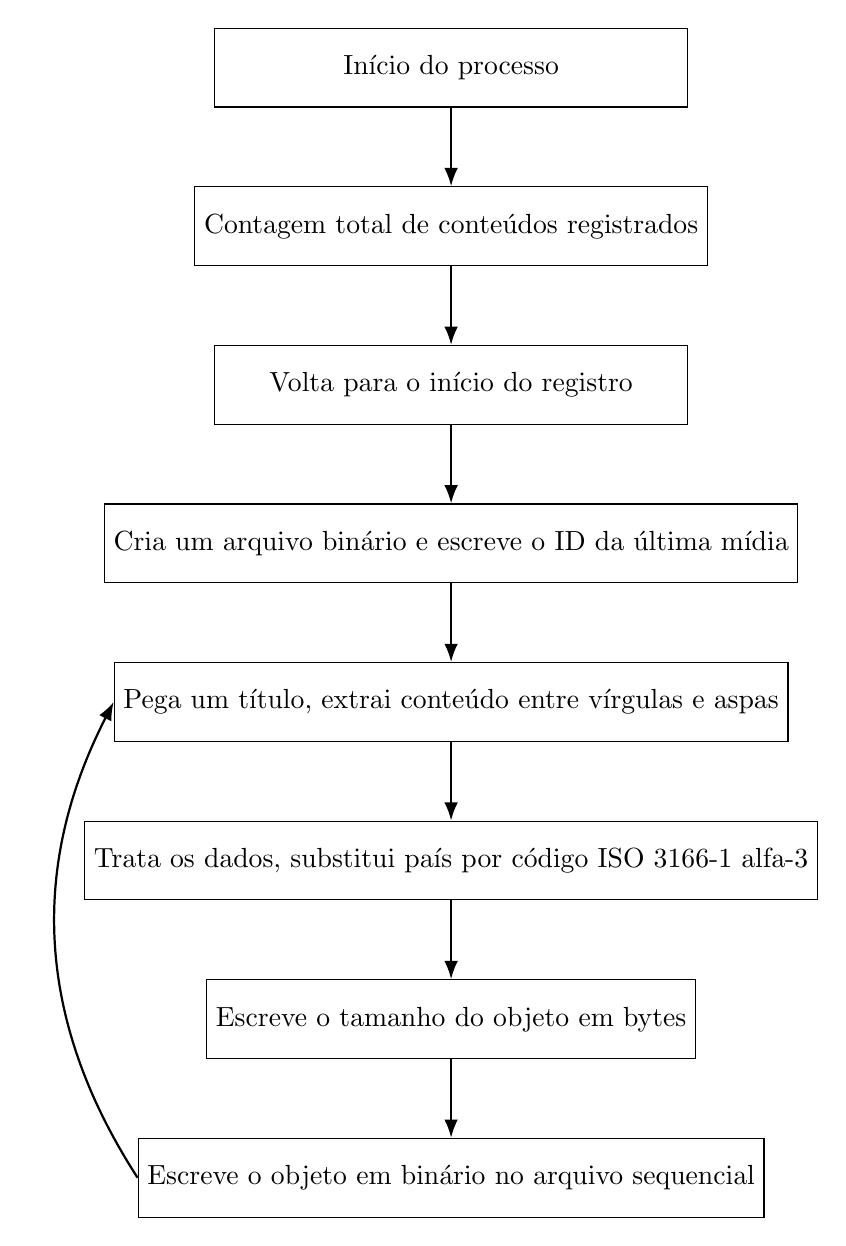
\begin{tikzpicture}[
    node distance=1cm,
    box/.style={draw, rectangle, minimum width=6cm, minimum height=1cm, align=center},
    arrow/.style={-{Latex}, thick}
]

% Etapa 0 (acima da primeira)
\node[box] (step0) {Início do processo};

\node[box, below=of step0] (step1) {Contagem total de conteúdos registrados};
\node[box, below=of step1] (step2) {Volta para o início do registro};
\node[box, below=of step2] (step3) {Cria um arquivo binário e escreve o ID da última mídia};
\node[box, below=of step3] (step4) {Pega um título, extrai conteúdo entre vírgulas e aspas};
\node[box, below=of step4] (step5) {Trata os dados, substitui país por código ISO 3166-1 alfa-3};
\node[box, below=of step5] (step6) {Escreve o tamanho do objeto em bytes};
\node[box, below=of step6] (step7) {Escreve o objeto em binário no arquivo sequencial};

% Setas diretas
\draw[arrow] (step0) -- (step1);
\draw[arrow] (step1) -- (step2);
\draw[arrow] (step2) -- (step3);
\draw[arrow] (step3) -- (step4);
\draw[arrow] (step4) -- (step5);
\draw[arrow] (step5) -- (step6);
\draw[arrow] (step6) -- (step7);

% Loop de retorno ao passo 0
\draw[arrow, bend left=30] (step7.west) to (step4.west);

\end{tikzpicture}
\end{center}



\section*{Codigo JAVA}
\begin{lstlisting}

 // Contagem dos registros do arquivo de filmes
        try (BufferedReader contagem = new BufferedReader(new FileReader(file))) {
            contagem.readLine(); // Pula o cabeçalho
            while (contagem.readLine() != null) {
                contador++;
            }
        } catch (IOException e) {
            System.out.println("Erro ao contar registros: " + e.getMessage());
            return;
        }
    
        // Processamento do arquivo de filmes
        try (
            BufferedReader leitura = new BufferedReader(new FileReader(file));
            RandomAccessFile out = new RandomAccessFile(binarioFile, "rw");
        ) {

            File fileExistente = new File(binarioFile);
            if (fileExistente.exists()) {
                fileExistente.delete(); // Exclui o arquivo existente
            }
            
            leitura.readLine(); // Pula o cabeçalho
            out.writeInt(contador); // Escreve o número total de registros no início do arquivo
    
            String line;
            int registro = 0;

            while ((line = leitura.readLine()) != null) {
                // Limpeza da linha para remover caracteres indesejados
                line = line.replaceAll(";", "").trim();
                line = line.replaceAll("^\"|\"$", "").trim();
                line = line.replaceAll("\"\"", "\"").trim();
    
                List<String> dadosFilme = extrairDadosLinha(line);
    
                // Substitui o nome do país pelo código correspondente
                String paisFilme = dadosFilme.get(4);
                dadosFilme.set(4, Pesquisar.PesquisarPaisAbre(binarioPais, paisFilme));
                registro++;
    
                // Criação do objeto Filme
                Filmes tmp = new Filmes(dadosFilme, registro, false);
    
                // Serializa o objeto Filme em bytes
                ByteArrayOutputStream baos = new ByteArrayOutputStream();
                try (ObjectOutputStream oos = new ObjectOutputStream(baos)) {
                    oos.writeObject(tmp);
                }
                byte[] tmpSize = baos.toByteArray();

                long posicaoAtual = out.getFilePointer();
    
                // Escreve o tamanho do objeto serializado
                out.writeInt(tmpSize.length);
                
                // Escreve os bytes do objeto no arquivo binário
                out.write(tmpSize);

            }

\end{lstlisting}

\subsubsection{CRUD}
O CRUD e uma parte essencial de nosso trabalho sendo uma das maiores, nele o usuário pode pesquisar, inserir novos dados, editar dados existentes e apagar aqueles que não os interessa.Sendo implementada na forma de menus na qual o usuário escolhe o que fazer.

\section*{Pesquisa}
A Pesquisa e feita através do ID, que ao ser obtido e feito a pesquisa no arquivo binário e ao ser encontrado e mostra na tela 

\section*{Remoção}
Muito semelhante a pesquisa a remoção e feita de uma maneira bem simples, e feita uma pesquisa e que o conteúdo ser encontrado e salvo em uma variável temporária, e adicionado como "TRUE" na variável lapide, e por fim atualizado no arquivo binário, caso o ultimo Filme/Serie for excluído e atualizado o numero que mostra o ultimo ID

\section*{Atualização}
Ao usuário selecionar a atualização ele realiza uma pesquisa, e logo em seguida um sub-menu e apresentado a ele mostrando todas as opções que ele pode editar, sendo:

\begin{itemize}
  \item Nome
  \item Nome do Diretor
  \item Data de Adição ao Catalogo
  \item Ano de Lançamento
  \item Duração, sendo minutos para filmes e temporadas para series
  \item Gêneros
  \item Classificação
  \item Tipo, se e um filme ou serie
\end{itemize}

Apos a atualização, a função remoção e chamada para o antigo objeto que e apagado e o novo e inserido, atualizando também o numero que representa o ultimo objeto inserido. 
\section*{Inserção}
A inserção e feita de um método semelhante, apos o utilizador escolher essa opção e pedido com que insira os dados nesta ordem:

\begin{itemize}
  \item Nome
  \item Nome do Diretor
  \item Data de Adição ao Catalogo
  \item Ano de Lançamento
  \item Duração, sendo minutos para filmes e temporadas para series
  \item Gêneros
  \item Classificação
  \item Tipo, se e um filme ou serie
\end{itemize}

Como conclusão, o ID e obtido conseguindo através da soma do maior ID presente no arquivo com 1, e e mostrado na tela o resultado, alem disso e perguntado a pessoa se esta tudo correto caso esteja o objeto e adicionado ao arquivo binário e atualiza ID do ultimo objeto no arquivo, caso contrario a função atualização e chamada.

\subsubsection{Resultado}
Como resultado do arquivo sequencial e comum o arquivo binário ser menor do que o arquivo CSV original, no nosso trabalho o tamanho reduziu de 1304 KB para 1124 KB, uma redução de 24.81\%.Sendo CRUD outro fator de extrema importancia devido ao fato de que, a grande maioria dos arquivo tem muandnça, sejam elas a insercao de um novo dado, a remocao, a alteração e ate mesmo a leitura de um dado.

\subsection{TP2}

O TP2 tem como proposta a implementação de arquivos de indexação como arvore (Arvore B, B+ ou B*), índices (Hashing Estendido) e duas lista para funcionar com Lista Invertida utilizando tudo aquilo que foi implementado no TP1, so que ao invés de se trabalhar com 2 arquivos agora se trabalha com 3, o banco de dados, o arquivo binário e o arquivo de indexação .

\subsubsection{Arvore}
Nesta etapa, optamos pela utilização da árvore B+ devido à sua facilidade de implementação, versatilidade e alto desempenho. Esses dois últimos aspectos representam um diferencial importante, já que a árvore B+ permite que o número de filhos de cada nó seja definido pelo usuário, podendo variar de 2 até 100, o que proporciona maior flexibilidade conforme a necessidade do sistema.

Apesar de dinâmica, a implementação da árvore B+ ainda é um processo complexo que exige atenção. Em nosso projeto, estruturamos da seguinte forma: durante a leitura e escrita dos dados, no momento em que ocorre a gravação no arquivo binário, o código também escreve os mesmos dados em um arquivo destinado à árvore B+. Utilizamos os IDs como chaves e ponteiros que indicam a posição dos filhos no mesmo arquivo. Caso o nó não possua filhos, o ponteiro recebe o valor -1. Além disso, realizamos os devidos ajustes, como rotações e redistribuições, sempre que necessário, para manter a estrutura balanceada.

Na operação de busca, o usuário insere o ID desejado, e o código percorre a árvore até localizar o filme ou série correspondente. Caso o conteúdo não seja encontrado, é exibida uma mensagem de erro. A remoção também se baseia na busca: após localizar o conteúdo, ele é excluído do arquivo e os ponteiros da árvore são atualizados adequadamente.

Por fim, a inserção de novos registros reutiliza grande parte do processo de escrita já desenvolvido. Assim como no TP1, o usuário insere um novo objeto, e ele é adicionado tanto ao arquivo binário quanto à árvore B+, utilizando a mesma função de escrita, com os devidos ajustes na estrutura da árvore.

\section*{Fluxo de Processamento de Conteúdo - Leitura e Escrita}
\begin{center}
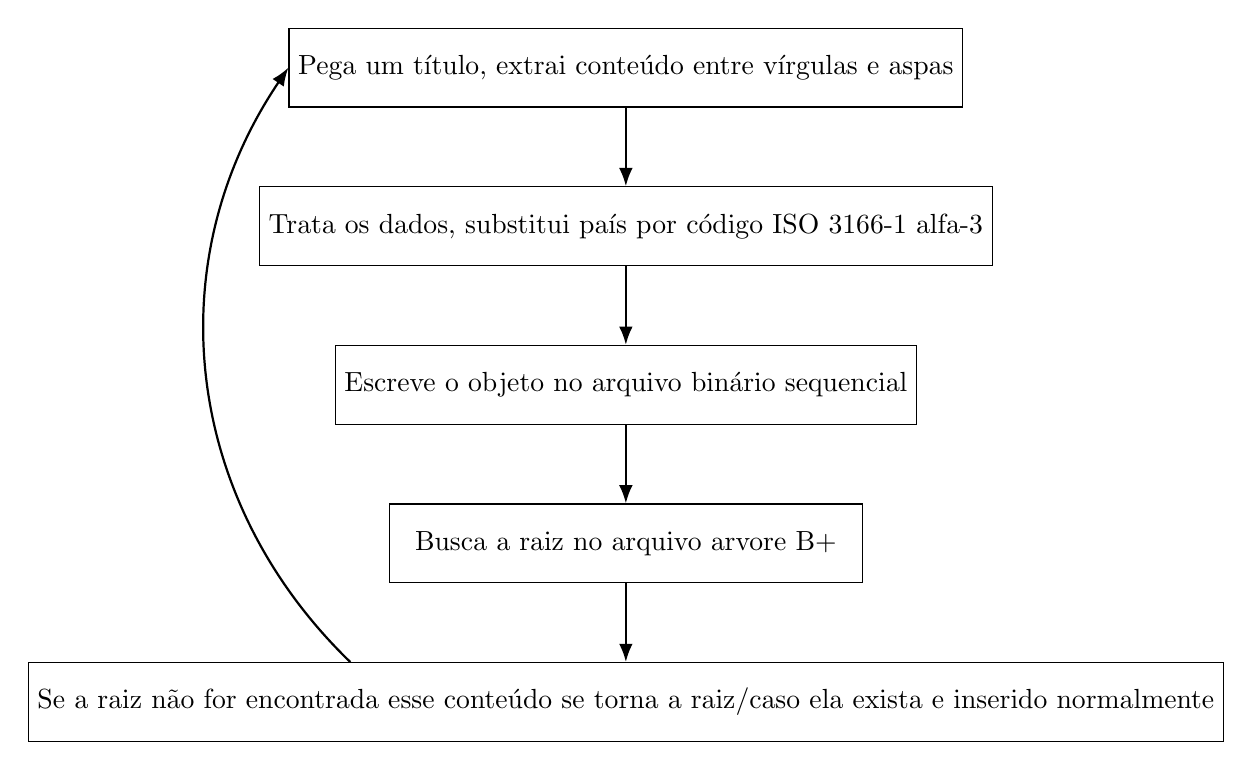
\begin{tikzpicture}[
    node distance=1cm,
    box/.style={draw, rectangle, minimum width=6cm, minimum height=1cm, align=center},
    arrow/.style={-{Latex}, thick}
]

% Etapa 0 (acima da primeira)
\node[box] (step0) {Pega um título, extrai conteúdo entre vírgulas e aspas};
\node[box, below=of step0] (step1) {Trata os dados, substitui país por código ISO 3166-1 alfa-3};
\node[box, below=of step1] (step2) {Escreve o objeto no arquivo binário sequencial};
\node[box, below=of step2] (step3) {Busca a raiz no arquivo arvore B+};
\node[box, below=of step3] (step4) {Se a raiz não for encontrada esse conteúdo se torna a raiz/caso ela exista e inserido normalmente};

% Setas diretas
\draw[arrow] (step0) -- (step1);
\draw[arrow] (step1) -- (step2);
\draw[arrow] (step2) -- (step3);
\draw[arrow] (step3) -- (step4);

% Loop de retorno ao passo 0
\draw[arrow, bend left=40] ([xshift=-3.5cm]step4.north) to (step0.west);

\end{tikzpicture}
\end{center}

\section*{Fluxo de Processamento de Conteúdo - Pesquisa}
\begin{center}
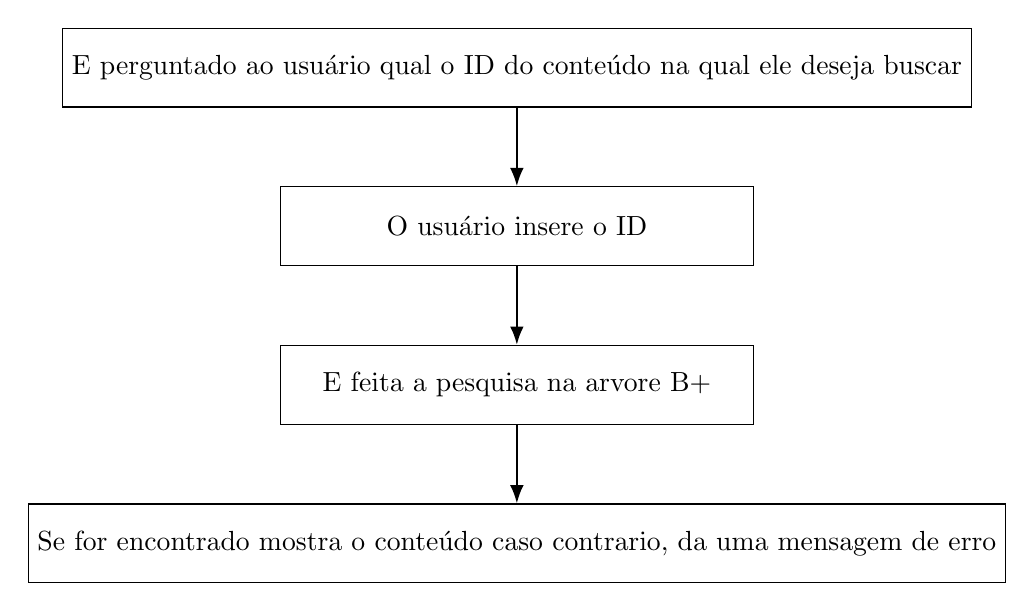
\begin{tikzpicture}[
    node distance=1cm,
    box/.style={draw, rectangle, minimum width=6cm, minimum height=1cm, align=center},
    arrow/.style={-{Latex}, thick}
]

% Etapa 0 (acima da primeira)
\node[box] (step0) {E perguntado ao usuário qual o ID do conteúdo na qual ele deseja buscar};
\node[box, below=of step0] (step1) {O usuário insere o ID};
\node[box, below=of step1] (step2) {E feita a pesquisa na arvore B+};
\node[box, below=of step2] (step3) {Se for encontrado mostra o conteúdo caso contrario, da uma mensagem de erro};

% Setas diretas
\draw[arrow] (step0) -- (step1);
\draw[arrow] (step1) -- (step2);
\draw[arrow] (step2) -- (step3);

\end{tikzpicture}
\end{center}

\section*{Fluxo de Processamento de Conteúdo - Remoção}
\begin{center}
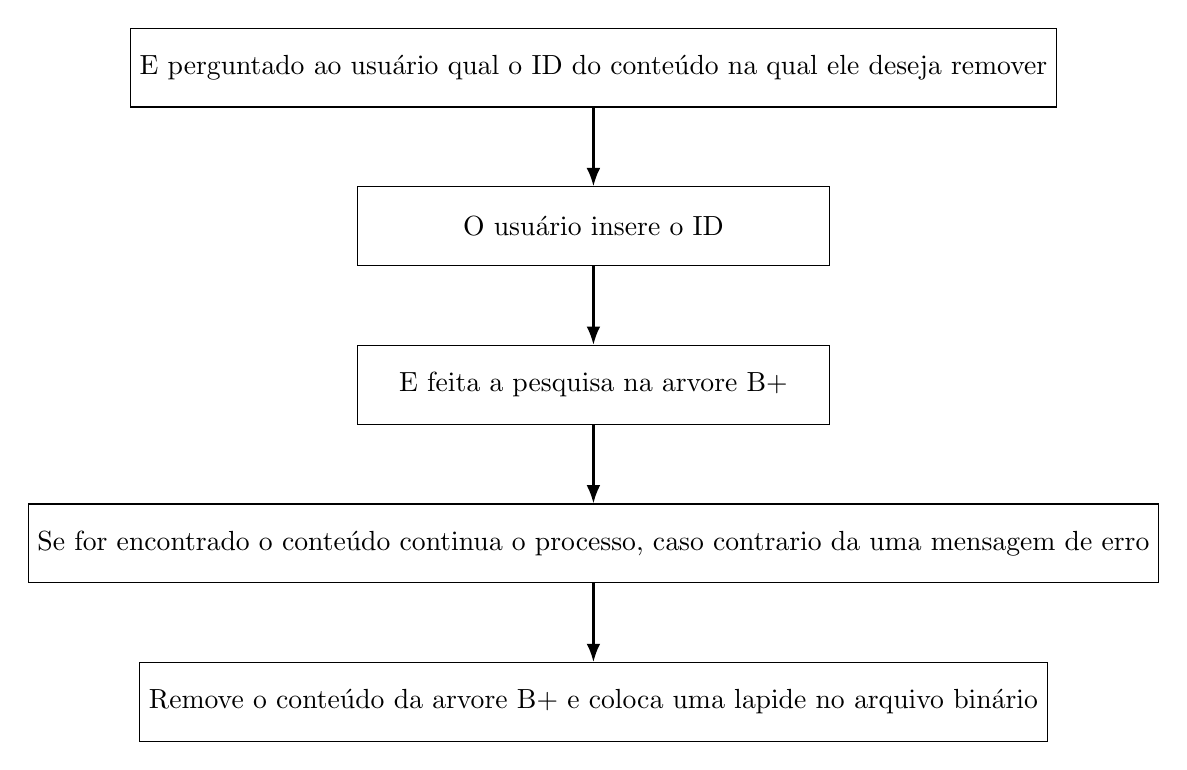
\begin{tikzpicture}[
    node distance=1cm,
    box/.style={draw, rectangle, minimum width=6cm, minimum height=1cm, align=center},
    arrow/.style={-{Latex}, thick}
]

% Etapa 0 (acima da primeira)
\node[box] (step0) {E perguntado ao usuário qual o ID do conteúdo na qual ele deseja remover};
\node[box, below=of step0] (step1) {O usuário insere o ID};
\node[box, below=of step1] (step2) {E feita a pesquisa na arvore B+};
\node[box, below=of step2] (step3) {Se for encontrado o conteúdo continua o processo, caso contrario da uma mensagem de erro};
\node[box, below=of step3] (step4) {Remove o conteúdo da arvore B+ e coloca uma lapide no arquivo binário};

% Setas diretas
\draw[arrow] (step0) -- (step1);
\draw[arrow] (step1) -- (step2);
\draw[arrow] (step2) -- (step3);
\draw[arrow] (step3) -- (step4);

\end{tikzpicture}
\end{center}

\section*{Fluxo de Processamento de Conteúdo - Adição}
\begin{center}
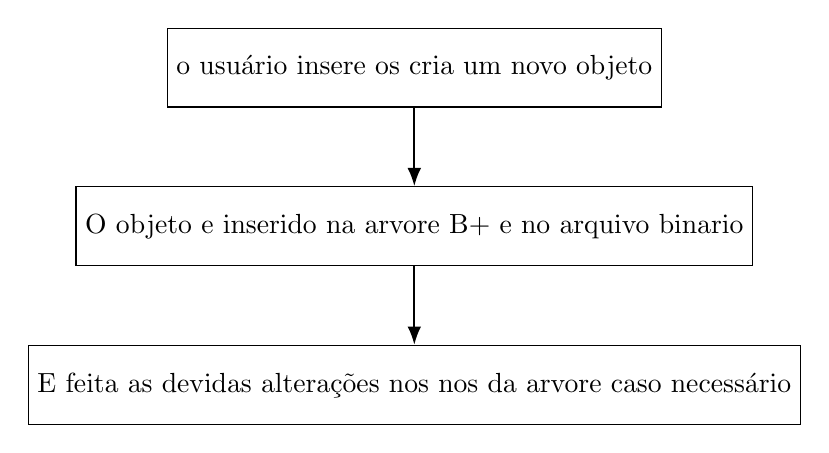
\begin{tikzpicture}[
    node distance=1cm,
    box/.style={draw, rectangle, minimum width=6cm, minimum height=1cm, align=center},
    arrow/.style={-{Latex}, thick}
]

% Etapa 0 (acima da primeira)
\node[box] (step0) {o usuário insere os cria um novo objeto};
\node[box, below=of step0] (step1) {O objeto e inserido na arvore B+ e  no arquivo binario};
\node[box, below=of step1] (step2) {E feita as devidas alterações nos nos da arvore caso necessário};


% Setas diretas
\draw[arrow] (step0) -- (step1);
\draw[arrow] (step1) -- (step2);

\end{tikzpicture}
\end{center}

\subsubsection{Hashing Estendido}

O hash extensível se destaca por evitar colisões de forma eficiente e por permitir que a estrutura se expanda conforme a necessidade, sem desperdício significativo de espaço.

Em nosso projeto, a implementação do hash extensível foi estruturada da seguinte forma: ao realizar a gravação de um novo registro no arquivo binário, o código também insere o mesmo registro em arquivos específicos do hash, utilizando o ID como chave. O diretório do hash armazena ponteiros para os cestos, que são responsáveis por guardar os registros. Cada cesto possui uma profundidade local, e o diretório possui uma profundidade global, permitindo que a estrutura se ajuste automaticamente conforme a quantidade de dados aumenta.

Quando um cesto atinge sua capacidade máxima, o diretório pode ser duplicado e os cestos redistribuídos, garantindo que a performance das operações seja mantida mesmo com grandes volumes de dados. Durante a busca, o usuário informa o ID desejado, e o algoritmo calcula o hash para localizar rapidamente o cesto correspondente e, em seguida, o registro. Caso o registro não seja encontrado, uma mensagem de erro é exibida.

A remoção de registros segue o mesmo princípio: o sistema localiza o cesto pelo hash do ID e remove o registro, atualizando o cesto no arquivo. A inserção de novos registros reutiliza parte do processo de escrita, garantindo que tanto o arquivo binário quanto a estrutura de hash estejam sempre sincronizados.

Dessa forma, o hash extensível proporciona uma solução eficiente, flexível e escalável para a indexação e gerenciamento dos registros no sistema, facilitando operações rápidas e seguras mesmo com grandes volumes de dados.

\section*{Fluxo de Processamento de Conteúdo - Leitura e Escrita (Hash Extensível)} 
\begin{center} 
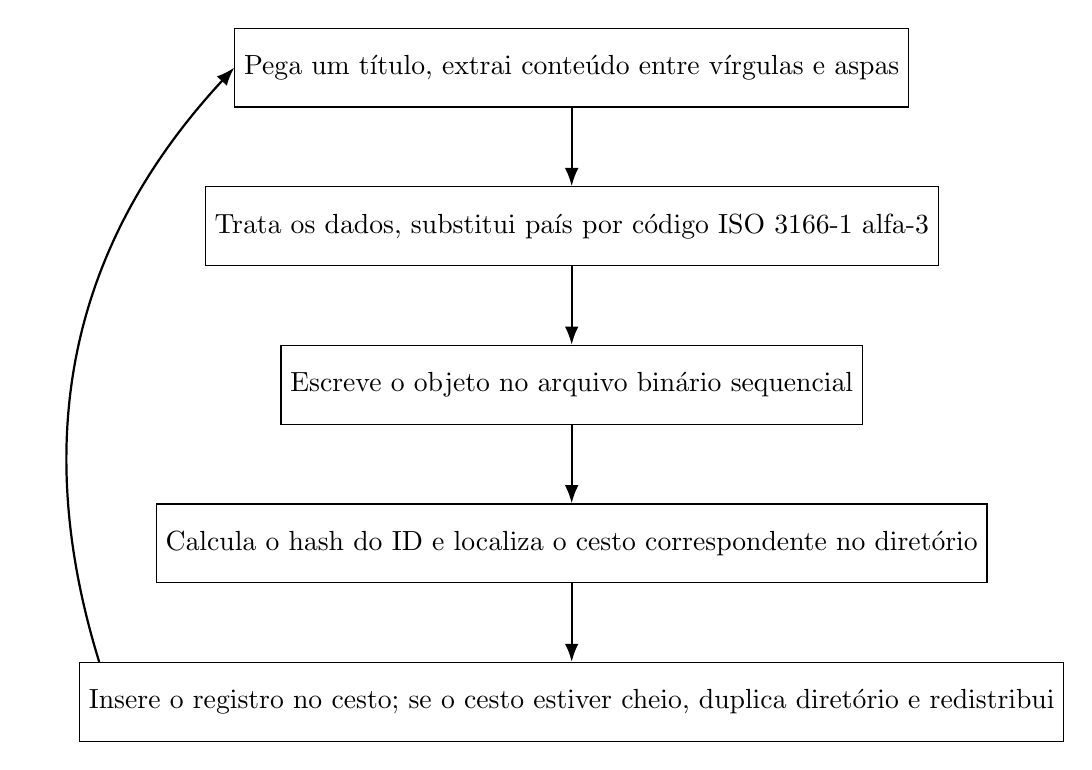
\begin{tikzpicture}[ 
node distance=1cm, 
box/.style={draw, rectangle, 
minimum width=6cm, minimum height=1cm, 
align=center}, 
arrow/.style={-{Latex}, thick} 
]

\node[box] (step0) {Pega um título, extrai conteúdo entre vírgulas e aspas};
\node[box, below=of step0] (step1) {Trata os dados, substitui país por código ISO 3166-1 alfa-3}; 
\node[box, below=of step1] (step2) {Escreve o objeto no arquivo binário sequencial}; 
\node[box, below=of step2] (step3) {Calcula o hash do ID e localiza o cesto correspondente no diretório}; 
\node[box, below=of step3] (step4) {Insere o registro no cesto; se o cesto estiver cheio, duplica diretório e redistribui};

\draw[arrow] (step0) -- (step1); 
\draw[arrow] (step1) -- (step2); 
\draw[arrow] (step2) -- (step3); 
\draw[arrow] (step3) -- (step4); 
\draw[arrow, bend left=30] ([xshift=-6cm]step4.north) to (step0.west);

\end{tikzpicture} 
\end{center}

\section*{Fluxo de Processamento de Conteúdo - Pesquisa (Hash Extensível)} 
\begin{center} 
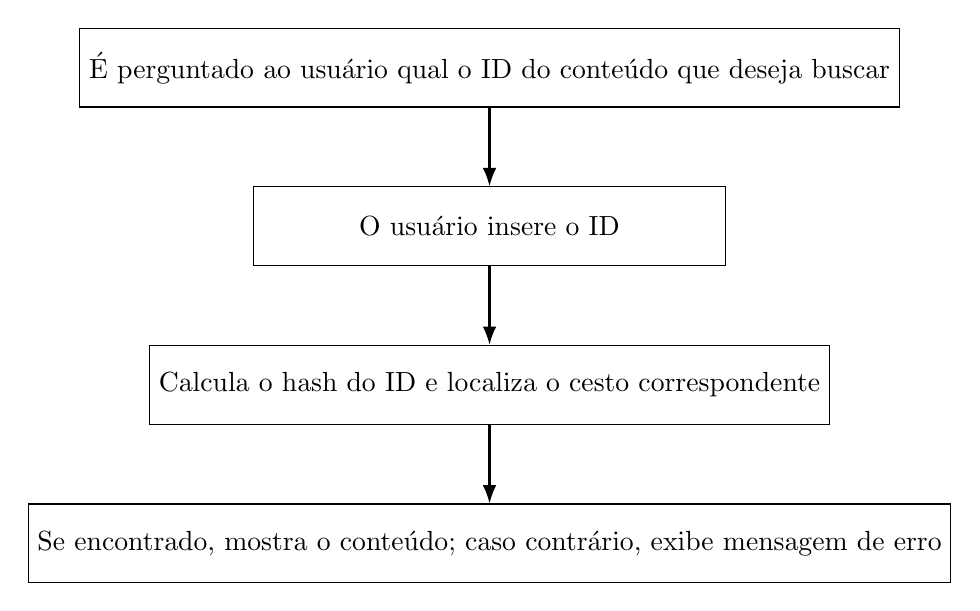
\begin{tikzpicture}[ 
node distance=1cm, 
box/.style={draw, 
rectangle, 
minimum width=6cm, 
minimum height=1cm, 
align=center}, 
arrow/.style={-{Latex}, thick} 
]

\node[box] (step0) {É perguntado ao usuário qual o ID do conteúdo que deseja buscar}; 
\node[box, below=of step0] (step1) {O usuário insere o ID}; 
\node[box, below=of step1] (step2) {Calcula o hash do ID e localiza o cesto correspondente}; 
\node[box, below=of step2] (step3) {Se encontrado, mostra o conteúdo; caso contrário, exibe mensagem de erro};

\draw[arrow] (step0) -- (step1); 
\draw[arrow] (step1) -- (step2); 
\draw[arrow] (step2) -- (step3);

\end{tikzpicture} 
\end{center}

\section*{Fluxo de Processamento de Conteúdo - Remoção (Hash Extensível)} 
\begin{center} 
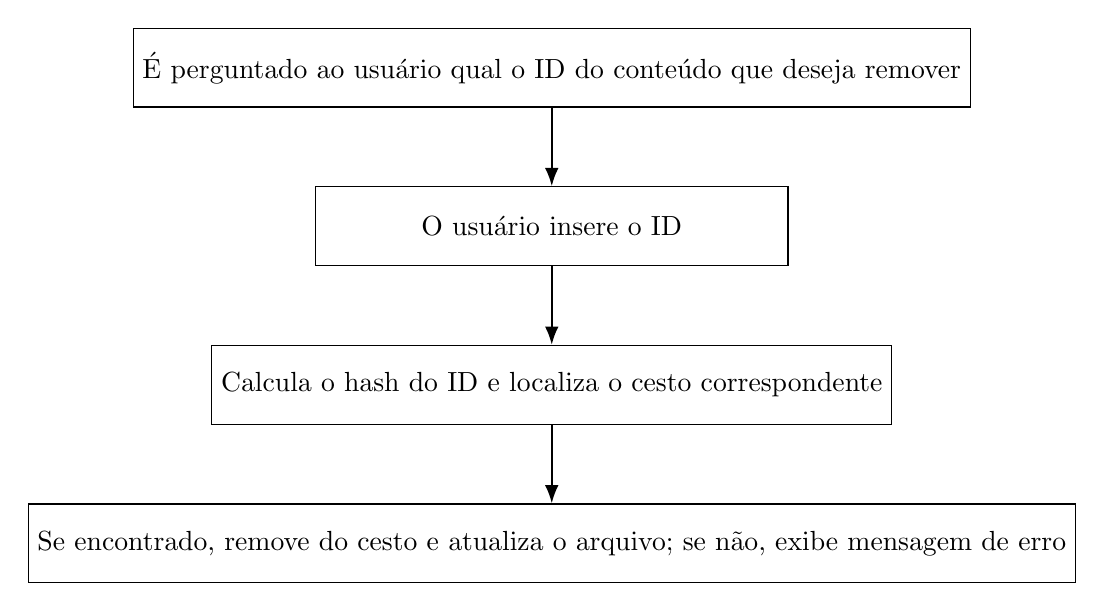
\begin{tikzpicture}[ 
node distance=1cm, 
box/.style={draw, rectangle, 
minimum width=6cm, 
minimum height=1cm, align=center}, 
arrow/.style={-{Latex}, thick} 
]

\node[box] (step0) {É perguntado ao usuário qual o ID do conteúdo que deseja remover}; 
\node[box, below=of step0] (step1) {O usuário insere o ID}; 
\node[box, below=of step1] (step2) {Calcula o hash do ID e localiza o cesto correspondente}; 
\node[box, below=of step2] (step3) {Se encontrado, remove do cesto e atualiza o arquivo; se não, exibe mensagem de erro};

\draw[arrow] (step0) -- (step1); 
\draw[arrow] (step1) -- (step2); 
\draw[arrow] (step2) -- (step3);

\end{tikzpicture} 
\end{center}

\section*{Fluxo de Processamento de Conteúdo - Adição (Hash Extensível)} 
\begin{center} 
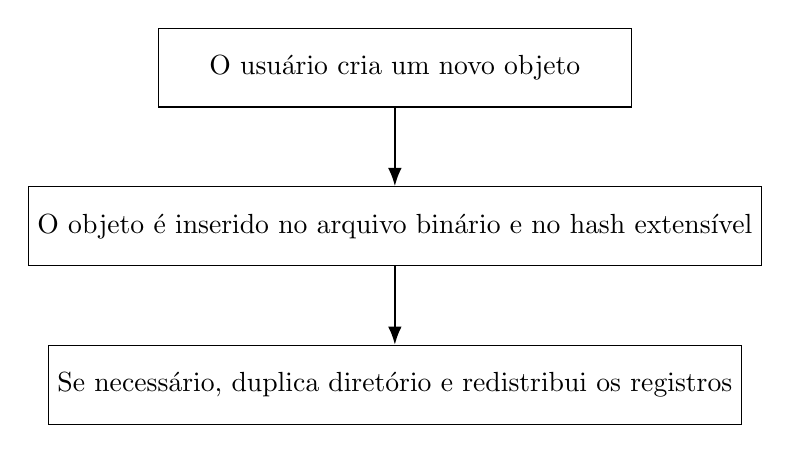
\begin{tikzpicture}[ 
node distance=1cm, 
box/.style={draw, rectangle, 
minimum width=6cm, 
minimum height=1cm, 
align=center}, 
arrow/.style={-{Latex}, thick} 
]

\node[box] (step0) {O usuário cria um novo objeto}; 
\node[box, below=of step0] (step1) {O objeto é inserido no arquivo binário e no hash extensível}; 
\node[box, below=of step1] (step2) {Se necessário, duplica diretório e redistribui os registros};

\draw[arrow] (step0) -- (step1); 
\draw[arrow] (step1) -- (step2);

\end{tikzpicture} 
\end{center}

\subsubsection{Lista Invertida}
A lista invertida se destaca por permitir a associação de uma chave (por exemplo, um termo, categoria ou atributo) a diversos registros, facilitando buscas rápidas e operações de filtragem em grandes volumes de dados.

Em nosso projeto, a lista invertida foi estruturada da seguinte forma: para cada chave, escolhida pelo usuário entre essas opções:

\begin{itemize}
  \item Nome do Diretor
  \item Data de Adição ao Catalogo
  \item Ano de Lançamento
  \item Duração, sendo minutos para filmes e temporadas para series
  \item Gêneros
  \item Classificação
\end{itemize}

Mantemos um dicionário que armazena o nome da chave e um ponteiro para o início de uma lista de blocos. Cada bloco contém um conjunto de elementos, onde cada elemento representa um ID e sua localização no arquivo de dados principal. Os blocos são encadeados, permitindo que a lista cresça dinamicamente conforme a quantidade de registros associados à chave aumenta. Caso um bloco atinja sua capacidade máxima, um novo bloco é criado e encadeado ao anterior.

Durante a inserção de um novo registro, o sistema verifica se a chave já existe no dicionário. Se não existir, um novo bloco é criado e a chave é adicionada ao dicionário. O novo elemento é então inserido no bloco correspondente, mantendo a lista ordenada por ID para facilitar buscas e remoções. Se o bloco estiver cheio, um novo bloco é alocado e encadeado à lista existente.

Na operação de busca, o usuário informa a chave desejada, e o sistema percorre os blocos associados a essa chave, retornando todos os IDs e localizações correspondentes. Caso a chave não seja encontrada, uma lista vazia é retornada. A remoção de registros também é eficiente: o sistema localiza o bloco correspondente e remove o elemento desejado, reorganizando a lista conforme necessário.

Por fim, a lista invertida oferece flexibilidade para operações de exclusão global (removendo um ID de todas as chaves) e limpeza total de uma chave, além de permitir a impressão de todas as listas e seus elementos para fins de auditoria ou depuração. Essa estrutura garante alto desempenho em operações de leitura e escrita, sendo especialmente útil em cenários de indexação e busca reversa.

\section*{Fluxo de Processamento de Conteúdo - Leitura e Escrita (Lista Invertida)} 
\begin{center} 
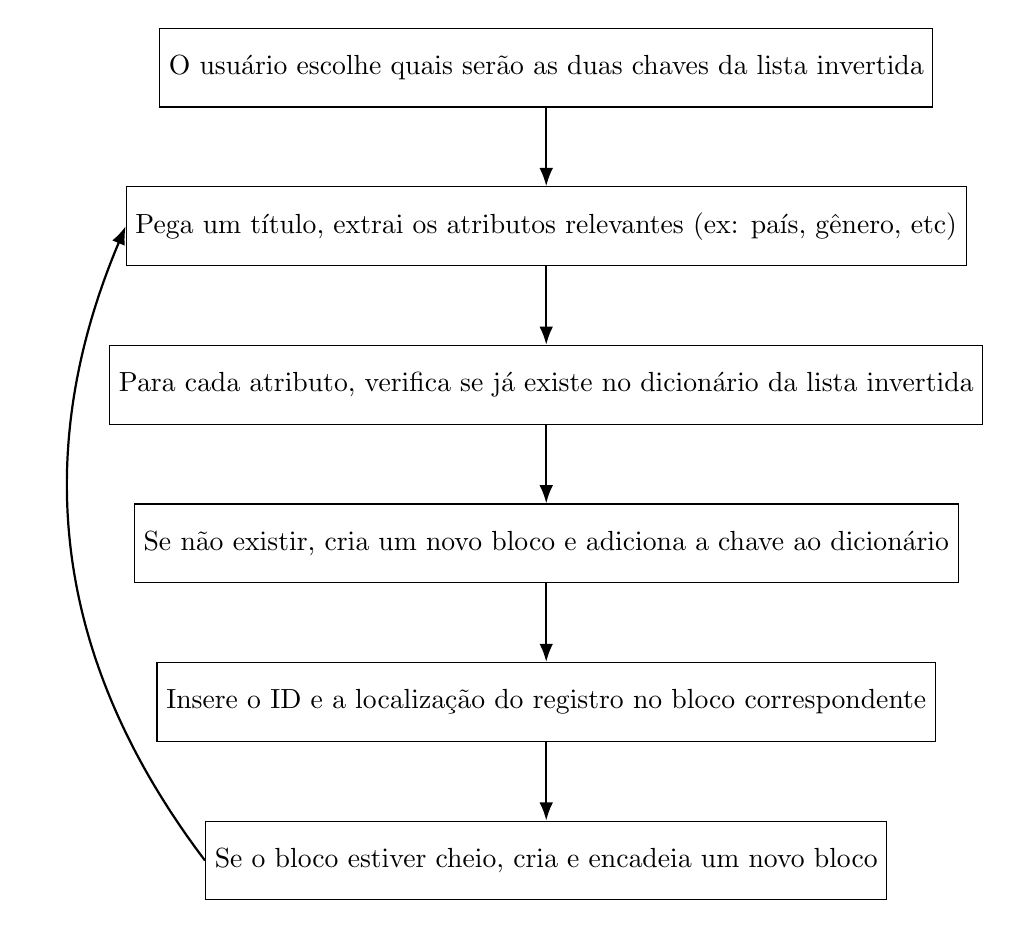
\begin{tikzpicture}[ 
node distance=1cm, 
box/.style={draw, rectangle, minimum width=6cm, minimum height=1cm, align=center}, 
arrow/.style={-{Latex}, thick} ]

\node[box] (step0) {O usuário escolhe quais serão as duas chaves da lista invertida};
\node[box, below=of step0] (step1) {Pega um título, extrai os atributos relevantes (ex: país, gênero, etc)};
\node[box, below=of step1] (step2) {Para cada atributo, verifica se já existe no dicionário da lista invertida}; 
\node[box, below=of step2] (step3) {Se não existir, cria um novo bloco e adiciona a chave ao dicionário}; 
\node[box, below=of step3] (step4) {Insere o ID e a localização do registro no bloco correspondente}; 
\node[box, below=of step4] (step5) {Se o bloco estiver cheio, cria e encadeia um novo bloco};

\draw[arrow] (step0) -- (step1);
\draw[arrow] (step1) -- (step2); 
\draw[arrow] (step2) -- (step3); 
\draw[arrow] (step3) -- (step4); 
\draw[arrow] (step4) -- (step5);

\draw[arrow, bend left=30] (step5.west) to (step1.west);

\end{tikzpicture} 
\end{center}

\section*{Fluxo de Processamento de Conteúdo - Pesquisa (Lista Invertida)} 
\begin{center} 
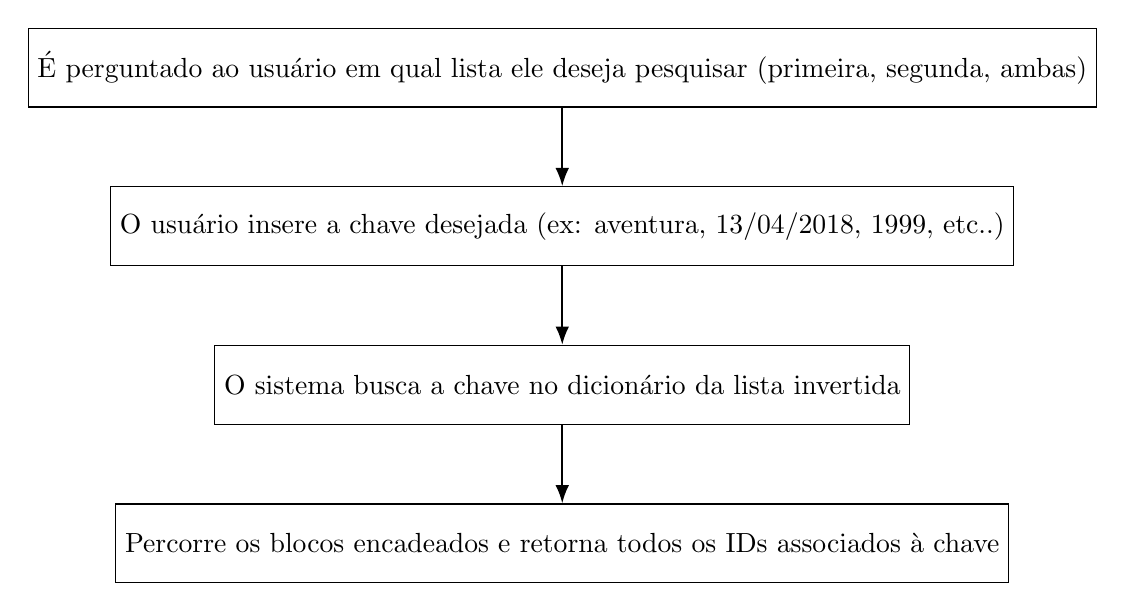
\begin{tikzpicture}[ 
node distance=1cm, 
box/.style={draw, 
rectangle, 
minimum width=6cm, 
minimum height=1cm, 
align=center}, 
arrow/.style={-{Latex}, thick} 
]

\node[box] (step0) {É perguntado ao usuário em qual lista ele deseja pesquisar (primeira, segunda, ambas)}; 
\node[box, below=of step0] (step1) {O usuário insere a chave desejada (ex: aventura, 13/04/2018, 1999, etc..)}; 
\node[box, below=of step1] (step2) {O sistema busca a chave no dicionário da lista invertida}; 
\node[box, below=of step2] (step3) {Percorre os blocos encadeados e retorna todos os IDs associados à chave};

\draw[arrow] (step0) -- (step1); 
\draw[arrow] (step1) -- (step2); 
\draw[arrow] (step2) -- (step3);

\end{tikzpicture} 
\end{center}

\section*{Fluxo de Processamento de Conteúdo - Remoção (Lista Invertida)} 
\begin{center} 
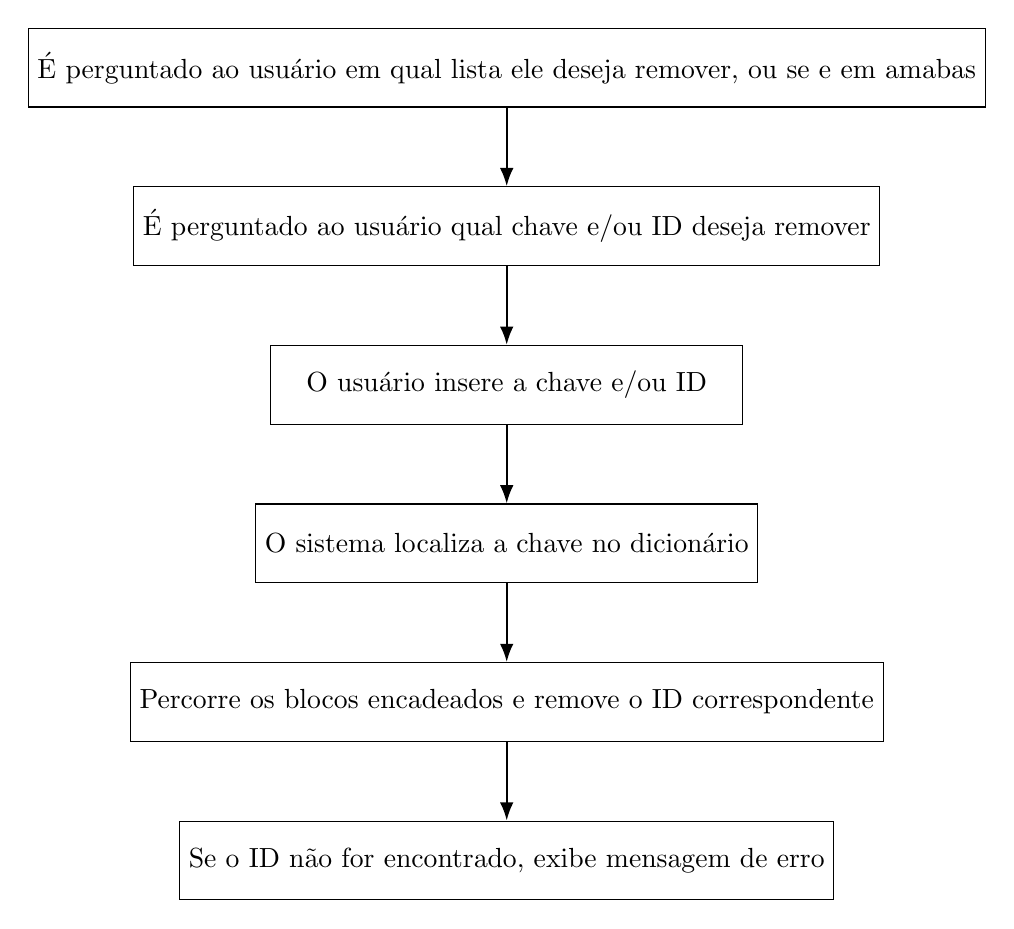
\begin{tikzpicture}[ 
node distance=1cm, 
box/.style={draw, 
rectangle, 
minimum width=6cm, 
minimum height=1cm, 
align=center}, 
arrow/.style={-{Latex}, thick} ]

\node[box] (step-1) {É perguntado ao usuário em qual lista ele deseja remover, ou se e em amabas}; 
\node[box, below=of step-1] (step0) {É perguntado ao usuário qual chave e/ou ID deseja remover}; 
\node[box, below=of step0] (step1) {O usuário insere a chave e/ou ID}; 
\node[box, below=of step1] (step2) {O sistema localiza a chave no dicionário}; 
\node[box, below=of step2] (step3) {Percorre os blocos encadeados e remove o ID correspondente}; 
\node[box, below=of step3] (step4) {Se o ID não for encontrado, exibe mensagem de erro};

\draw[arrow] (step-1) -- (step0); 
\draw[arrow] (step0) -- (step1); 
\draw[arrow] (step1) -- (step2); 
\draw[arrow] (step2) -- (step3); 
\draw[arrow] (step3) -- (step4);

\end{tikzpicture} 
\end{center}

\section*{Fluxo de Processamento de Conteúdo - Adição (Lista Invertida)} 
\begin{center} 
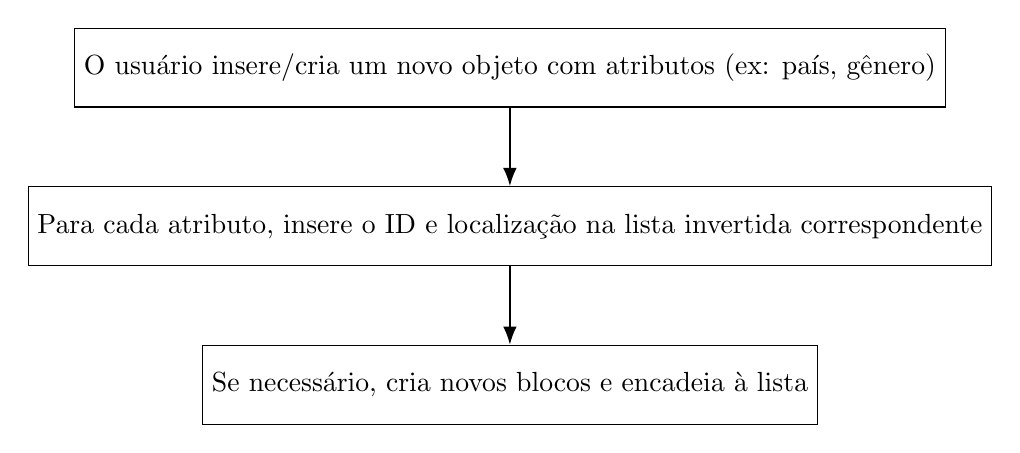
\begin{tikzpicture}[ 
node distance=1cm, 
box/.style={draw, rectangle, 
minimum width=6cm, 
minimum height=1cm, 
align=center}, 
arrow/.style={-{Latex}, thick} 
]

\node[box] (step0) {O usuário insere/cria um novo objeto com atributos (ex: país, gênero)}; 
\node[box, below=of step0] (step1) {Para cada atributo, insere o ID e localização na lista invertida correspondente}; 
\node[box, below=of step1] (step2) {Se necessário, cria novos blocos e encadeia à lista};

\draw[arrow] (step0) -- (step1); 
\draw[arrow] (step1) -- (step2);

\end{tikzpicture} 
\end{center}

\subsubsection{Resultado}
Como resultado da implementação de arquivos de indexação melhoramos em muito o tempo que se leva para buscar conteúdos em uma maneira eficiente, que comparado a anterior gasta muito menos recurso computacional.

\subsection{TP3}
Esta parte tem como proposta a implementação de compactação e descompactação de dados, utilizando Huffman e LZW, além de dois métodos de casamento de padrões, na parte já existente do código.

\subsubsection{Compactação e Descompactação}
\subsection*{Huffman}
O principal diferencial do Huffman é sua capacidade de reduzir o tamanho dos arquivos ao atribuir códigos menores para os bytes mais frequentes, proporcionando uma compressão eficiente e sem perdas, o que é fundamental para otimizar o armazenamento e a transmissão de informações no sistema.

A implementação do algoritmo de Huffman, necessita de atenção em detalhes como a construção da árvore de códigos e o mapeamento correto entre símbolos e seus códigos binários. Em nosso projeto, estruturamos o processo da seguinte forma: durante a leitura dos dados, o sistema calcula a frequência de cada byte presente no conteúdo a ser compactado. Com essas frequências, é construída uma árvore de Huffman, onde cada nó representa um símbolo e sua frequência, e os caminhos da raiz até as folhas determinam os códigos binários de cada símbolo.

No momento da escrita, cada byte do conteúdo original é substituído pelo seu respectivo código de Huffman, gerando uma sequência compactada de bits. Essa sequência é armazenada em um vetor de bits, reduzindo significativamente o espaço ocupado em disco. Para garantir a correta descompactação, a tabela de códigos gerada é mantida e utilizada posteriormente no processo inverso.

Na operação de descompactação, o sistema utiliza a tabela de códigos para reconstruir o conteúdo original a partir da sequência de bits compactada. O algoritmo percorre os bits, identificando os padrões correspondentes a cada símbolo, até restaurar completamente os dados originais. Caso haja qualquer inconsistência ou erro na sequência, uma mensagem de erro é exibida ao usuário.

Por fim, a integração do algoritmo de Huffman ao sistema foi realizada de forma transparente, permitindo que a compactação e descompactação dos dados ocorra automaticamente durante as operações de leitura e escrita, sem a necessidade de intervenção manual do usuário. Isso garante maior eficiência e praticidade no gerenciamento dos arquivos do projeto.

\section*{Fluxo de Processamento de Conteúdo - Compressão (Huffman)} 
\begin{center} 
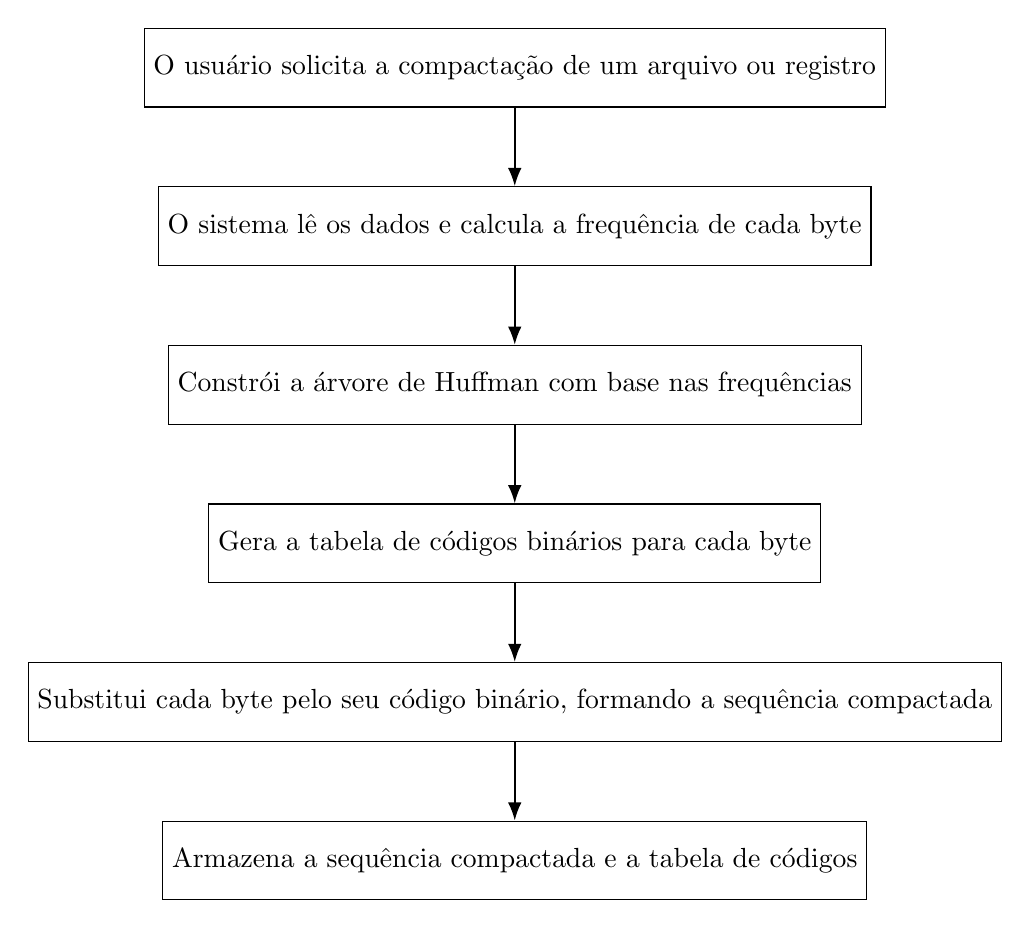
\begin{tikzpicture}[ 
node distance=1cm, 
box/.style={draw, 
rectangle, 
minimum width=6cm, 
minimum height=1cm, 
align=center}, 
arrow/.style={-{Latex}, thick} 
]

\node[box] (step0) {O usuário solicita a compactação de um arquivo ou registro}; 
\node[box, below=of step0] (step1) {O sistema lê os dados e calcula a frequência de cada byte}; 
\node[box, below=of step1] (step2) {Constrói a árvore de Huffman com base nas frequências}; 
\node[box, below=of step2] (step3) {Gera a tabela de códigos binários para cada byte}; 
\node[box, below=of step3] (step4) {Substitui cada byte pelo seu código binário, formando a sequência compactada}; 
\node[box, below=of step4] (step5) {Armazena a sequência compactada e a tabela de códigos};

\draw[arrow] (step0) -- (step1); 
\draw[arrow] (step1) -- (step2); 
\draw[arrow] (step2) -- (step3); 
\draw[arrow] (step3) -- (step4); 
\draw[arrow] (step4) -- (step5);

\end{tikzpicture} 
\end{center}

\section*{Fluxo de Processamento de Conteúdo - Descompressão (Huffman)} 
\begin{center} 
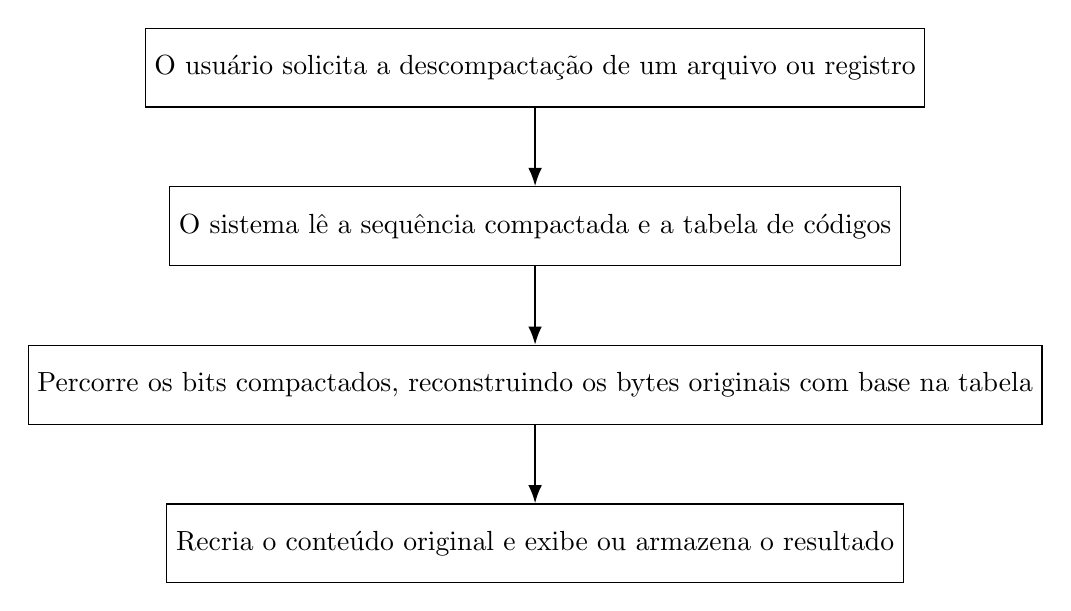
\begin{tikzpicture}[ 
node distance=1cm, 
box/.style={draw, 
rectangle, 
minimum width=6cm, 
minimum height=1cm, 
align=center}, 
arrow/.style={-{Latex}, thick} 
]

\node[box] (step0) {O usuário solicita a descompactação de um arquivo ou registro}; 
\node[box, below=of step0] (step1) {O sistema lê a sequência compactada e a tabela de códigos}; 
\node[box, below=of step1] (step2) {Percorre os bits compactados, reconstruindo os bytes originais com base na tabela}; 
\node[box, below=of step2] (step3) {Recria o conteúdo original e exibe ou armazena o resultado};

\draw[arrow] (step0) -- (step1); 
\draw[arrow] (step1) -- (step2); 
\draw[arrow] (step2) -- (step3);

\end{tikzpicture} 
\end{center}

\subsection*{LZW}
O LZW se destaca por não depender de tabelas de frequência prévias e por construir dinamicamente um dicionário durante o processo de compressão, o que proporciona flexibilidade e bons resultados para diferentes tipos de dados.

A implementação do LZW, exige atenção ao gerenciamento do dicionário e à manipulação dos índices de códigos. Em nosso projeto, estruturamos o processo da seguinte forma: durante a leitura dos dados, o sistema inicializa um dicionário contendo todas as possíveis sequências de um único byte. Em seguida, percorre o conteúdo a ser compactado, buscando sempre a maior sequência de bytes já presente no dicionário. Quando uma nova sequência é encontrada, ela é adicionada ao dicionário e o índice correspondente à última sequência conhecida é armazenado como parte da saída compactada.

No momento da escrita, os índices gerados são convertidos em uma sequência de bits, que é então armazenada em um vetor de bytes, reduzindo significativamente o espaço ocupado em disco. O tamanho dos índices é definido por uma constante, permitindo ajustar a quantidade máxima de entradas no dicionário conforme a necessidade do sistema.

Na operação de descompactação, o sistema reconstrói o dicionário de forma idêntica ao processo de compressão, utilizando os índices para recuperar as sequências originais de bytes. O algoritmo garante que, a cada novo índice lido, a sequência correspondente seja corretamente reconstruída e adicionada ao dicionário, restaurando fielmente o conteúdo original. Caso haja qualquer inconsistência ou erro na sequência de índices, uma mensagem de erro é exibida ao usuário.

Por fim, a integração do algoritmo LZW ao sistema foi realizada de forma transparente, permitindo que a compactação e descompactação dos dados ocorra automaticamente durante as operações de leitura e escrita, sem a necessidade de intervenção manual do usuário. Isso garante maior eficiência e praticidade no gerenciamento dos arquivos do projeto.

\section*{Fluxo de Processamento de Conteúdo - Compressão (LZW)} 
\begin{center} 
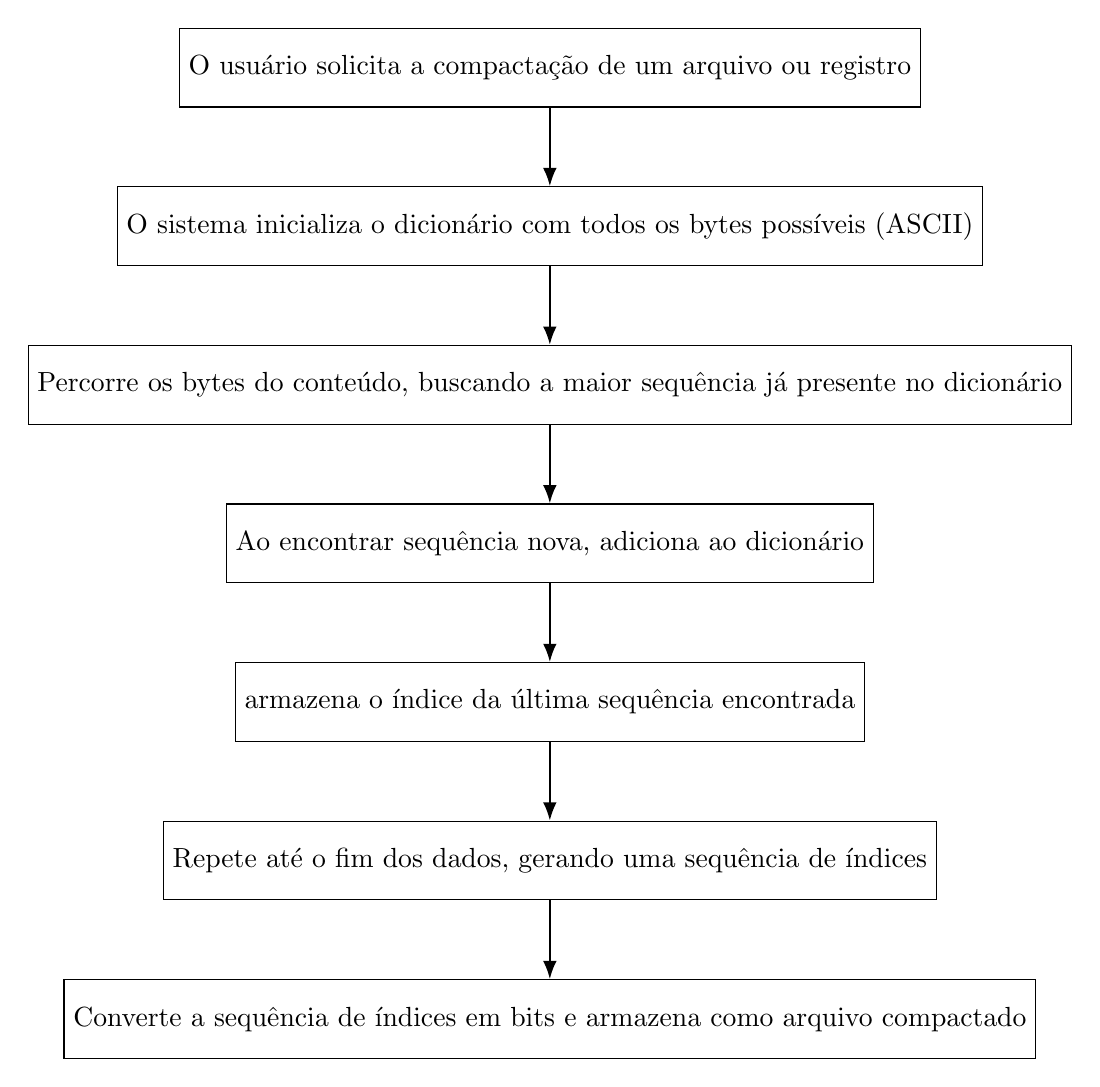
\begin{tikzpicture}[ 
node distance=1cm, 
box/.style={draw, 
rectangle, 
minimum width=6cm, 
minimum height=1cm, 
align=center}, 
arrow/.style={-{Latex}, thick} 
]

\node[box] (step0) {O usuário solicita a compactação de um arquivo ou registro}; 
\node[box, below=of step0] (step1) {O sistema inicializa o dicionário com todos os bytes possíveis (ASCII)}; 
\node[box, below=of step1] (step2) {Percorre os bytes do conteúdo, buscando a maior sequência já presente no dicionário}; 
\node[box, below=of step2] (step3) {Ao encontrar sequência nova, adiciona ao dicionário}; 
\node[box, below=of step3] (step4) {armazena o índice da última sequência encontrada}; 
\node[box, below=of step4] (step5) {Repete até o fim dos dados, gerando uma sequência de índices}; 
\node[box, below=of step5] (step6) {Converte a sequência de índices em bits e armazena como arquivo compactado};

\draw[arrow] (step0) -- (step1); 
\draw[arrow] (step1) -- (step2); 
\draw[arrow] (step2) -- (step3); 
\draw[arrow] (step3) -- (step4); 
\draw[arrow] (step4) -- (step5);
\draw[arrow] (step5) -- (step6);

\end{tikzpicture} 
\end{center}

\vspace{8cm}

\section*{Fluxo de Processamento de Conteúdo - Descompressão (LZW)} 
\begin{center} 
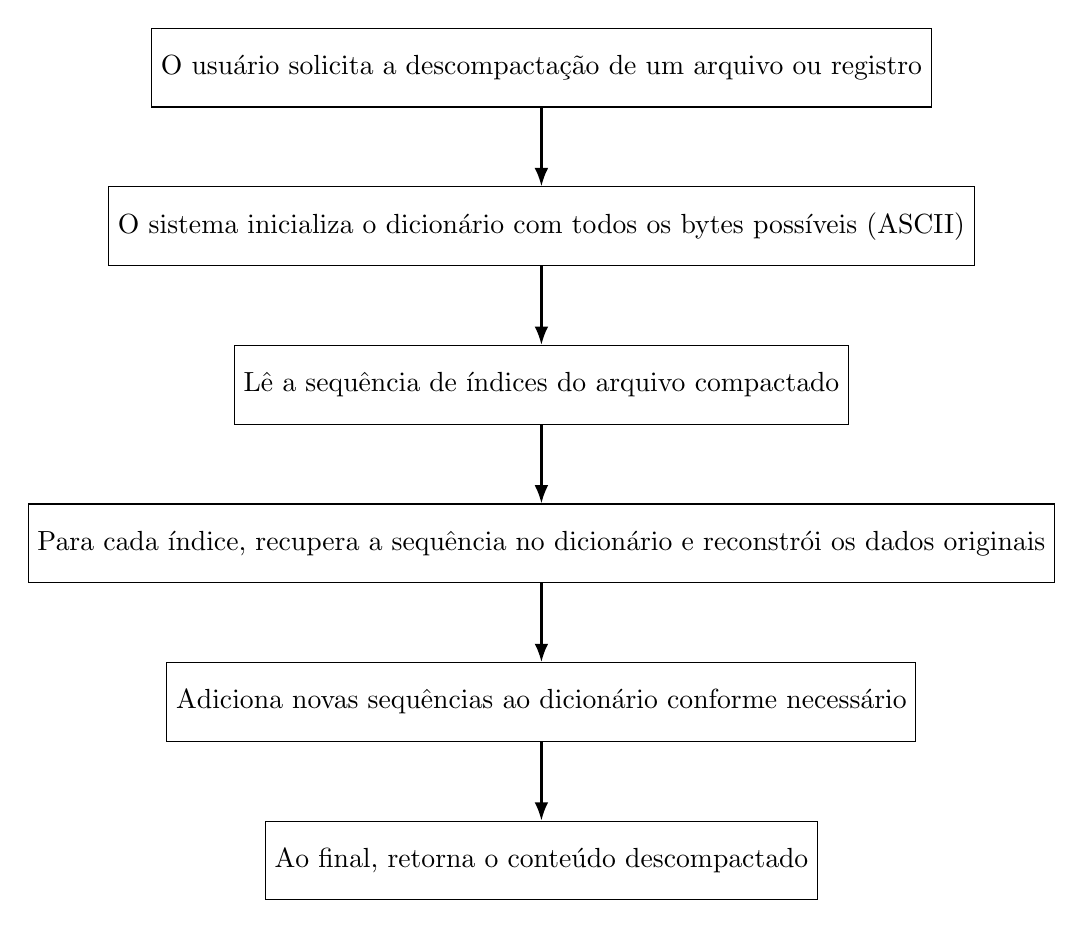
\begin{tikzpicture}[ 
node distance=1cm, 
box/.style={draw, 
rectangle, 
minimum width=6cm, 
minimum height=1cm, 
align=center}, 
arrow/.style={-{Latex}, thick} 
]

\node[box] (step0) {O usuário solicita a descompactação de um arquivo ou registro}; 
\node[box, below=of step0] (step1) {O sistema inicializa o dicionário com todos os bytes possíveis (ASCII)}; 
\node[box, below=of step1] (step2) {Lê a sequência de índices do arquivo compactado}; 
\node[box, below=of step2] (step3) {Para cada índice, recupera a sequência no dicionário e reconstrói os dados originais}; 
\node[box, below=of step3] (step4) {Adiciona novas sequências ao dicionário conforme necessário}; 
\node[box, below=of step4] (step5) {Ao final, retorna o conteúdo descompactado};

\draw[arrow] (step0) -- (step1); 
\draw[arrow] (step1) -- (step2); 
\draw[arrow] (step2) -- (step3); 
\draw[arrow] (step3) -- (step4); 
\draw[arrow] (step4) -- (step5);

\end{tikzpicture} 
\end{center}

\subsubsection{Casamento de Padrões}
Na implementações de padrões nos decidimos por optar pele escolha de Boyer Moore e KMP, devido ao foto de serem as mais simples além de ser aquelas na qual temos o maior conhecimento prévio sobre como funciona e como implementar.

\subsection*{Boyer Moore}
O principal diferencial do algoritmo de Boyer-Moore está em sua eficiência para buscas de padrões em grandes volumes de texto, utilizando heurísticas que permitem “saltos” inteligentes durante a varredura, reduzindo drasticamente o número de comparações necessárias. Isso é fundamental para acelerar pesquisas em arquivos extensos, como os utilizados no sistema.

A implementação do algoritmo de Boyer-Moore, embora baseada em conceitos clássicos, demanda atenção especial ao pré-processamento do padrão de busca. Em nosso projeto, esse processo consiste em calcular a última ocorrência de cada caractere presente no padrão, criando uma tabela que será utilizada para determinar o quanto o padrão pode ser deslocado no texto após uma falha de correspondência.

Durante a busca, o algoritmo compara o padrão com o texto da direita para a esquerda. Quando ocorre um descompasso entre os caracteres, a heurística do “caractere ruim” é aplicada: o padrão é deslocado de acordo com a posição da última ocorrência do caractere problemático, evitando comparações desnecessárias e tornando o processo muito mais rápido do que abordagens ingênuas.

No sistema, a busca por padrões é realizada diretamente sobre os registros dos filmes armazenados em arquivos binários. Para cada filme, os campos relevantes são extraídos e convertidos em texto, e o algoritmo de Boyer-Moore é aplicado para verificar a presença do padrão desejado. Caso o padrão seja encontrado, o registro correspondente é exibido ao usuário.

A integração do Boyer-Moore ao projeto foi feita de forma modular, permitindo que buscas eficientes sejam realizadas em diferentes campos dos registros, sem a necessidade de varrer todo o conteúdo byte a byte. Isso garante maior agilidade nas operações de pesquisa e contribui para uma experiência de uso mais fluida e responsiva no sistema.

\section*{Fluxo de Processamento de Conteúdo - Pesquisa (Boyer-Moore)} 
\begin{center} 
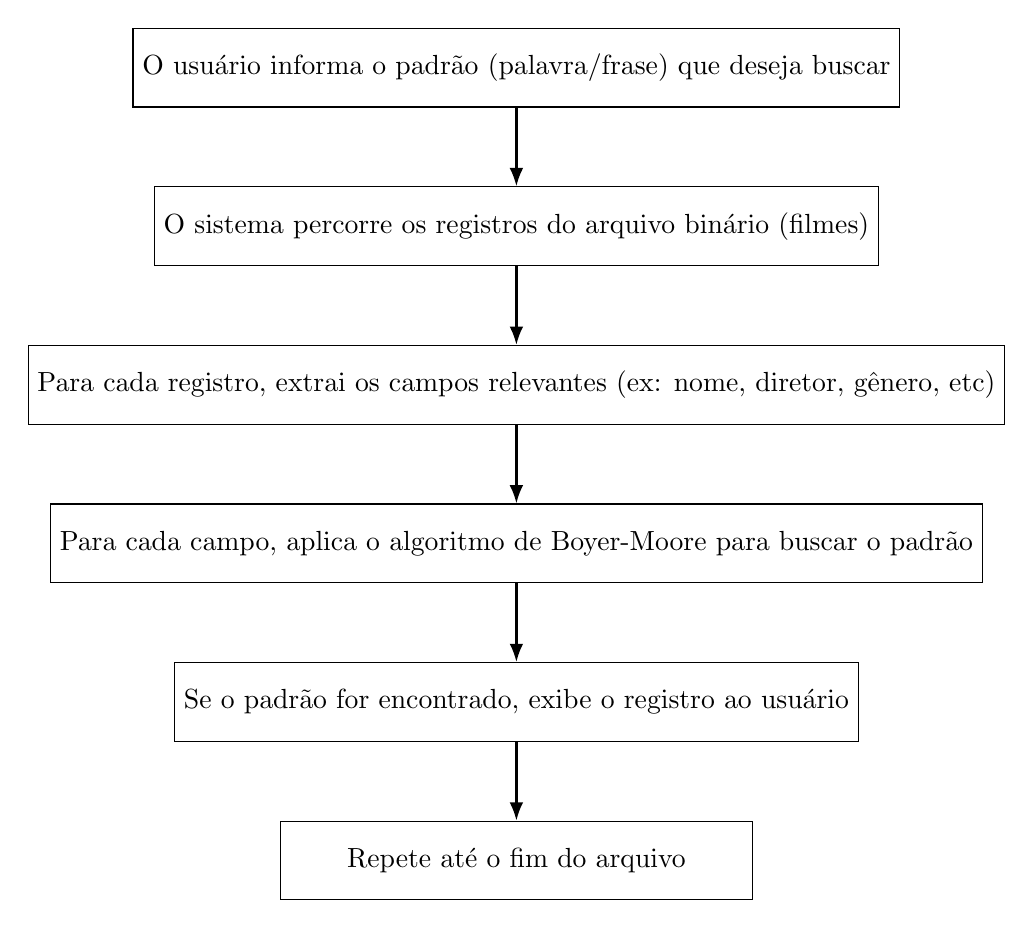
\begin{tikzpicture}[ 
node distance=1cm, 
box/.style={draw, 
rectangle, 
minimum width=6cm, 
minimum height=1cm, 
align=center}, 
arrow/.style={-{Latex}, thick} 
]

\node[box] (step0) {O usuário informa o padrão (palavra/frase) que deseja buscar}; 
\node[box, below=of step0] (step1) {O sistema percorre os registros do arquivo binário (filmes)}; 
\node[box, below=of step1] (step2) {Para cada registro, extrai os campos relevantes (ex: nome, diretor, gênero, etc)}; 
\node[box, below=of step2] (step3) {Para cada campo, aplica o algoritmo de Boyer-Moore para buscar o padrão}; 
\node[box, below=of step3] (step4) {Se o padrão for encontrado, exibe o registro ao usuário}; 
\node[box, below=of step4] (step5) {Repete até o fim do arquivo};

\draw[arrow] (step0) -- (step1); 
\draw[arrow] (step1) -- (step2); 
\draw[arrow] (step2) -- (step3); 
\draw[arrow] (step3) -- (step4); 
\draw[arrow] (step4) -- (step5);

\end{tikzpicture} 
\end{center}

\section*{Fluxo de Processamento de Conteúdo - Pré-processamento (Boyer-Moore)} 
\begin{center} 
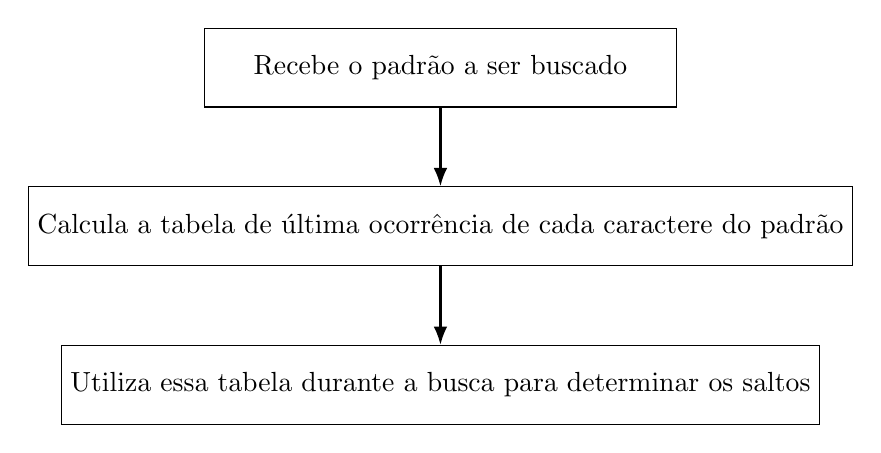
\begin{tikzpicture}[ node distance=1cm, 
box/.style={draw, 
rectangle, 
minimum width=6cm, 
minimum height=1cm, 
align=center}, 
arrow/.style={-{Latex}, thick} 
]

\node[box] (step0) {Recebe o padrão a ser buscado}; 
\node[box, below=of step0] (step1) {Calcula a tabela de última ocorrência de cada caractere do padrão}; 
\node[box, below=of step1] (step2) {Utiliza essa tabela durante a busca para determinar os saltos};

\draw[arrow] (step0) -- (step1); 
\draw[arrow] (step1) -- (step2);

\end{tikzpicture} 
\end{center}

\subsection*{KMP}
A grande vantagem do algoritmo KMP (Knuth-Morris-Pratt) é sua eficiência na busca de padrões em textos, evitando retrocessos desnecessários e tornando o processo de pesquisa muito mais rápido, especialmente em grandes volumes de dados. Isso é fundamental para otimizar buscas por informações específicas dentro dos registros do sistema.

A implementação do algoritmo KMP, embora baseada em um conceito simples, exige atenção ao pré-processamento do padrão de busca. Em nosso projeto, esse processo consiste na construção do vetor LPS (Longest Prefix Suffix), que armazena o tamanho do maior prefixo do padrão que também é sufixo. Esse vetor permite que, ao ocorrer uma falha na correspondência durante a busca, o algoritmo saiba exatamente para onde deve voltar no padrão, evitando comparações repetidas.

Durante a busca, o algoritmo compara o padrão com o texto de forma sequencial. Quando ocorre uma diferença entre os caracteres, o vetor LPS é utilizado para determinar o próximo ponto de comparação, sem a necessidade de reiniciar a busca do início do padrão. Isso garante que cada posição do texto seja analisada no máximo uma vez, proporcionando uma busca eficiente.

No sistema, a busca por padrões é realizada diretamente nos registros dos filmes armazenados em arquivos binários. Para cada filme, os campos relevantes são extraídos e convertidos em texto, e o algoritmo KMP é aplicado para verificar a presença do padrão desejado. Caso o padrão seja encontrado, o registro correspondente é exibido ao usuário.

A integração do KMP ao projeto foi feita de forma transparente, permitindo buscas rápidas e precisas em diferentes campos dos registros, sem a necessidade de varrer todo o conteúdo de forma ineficiente. Isso garante maior agilidade nas operações de pesquisa e contribui para uma experiência de uso mais eficiente e satisfatória no sistema.

\section*{Fluxo de Processamento de Conteúdo - Pesquisa (KMP)} 
\begin{center} 
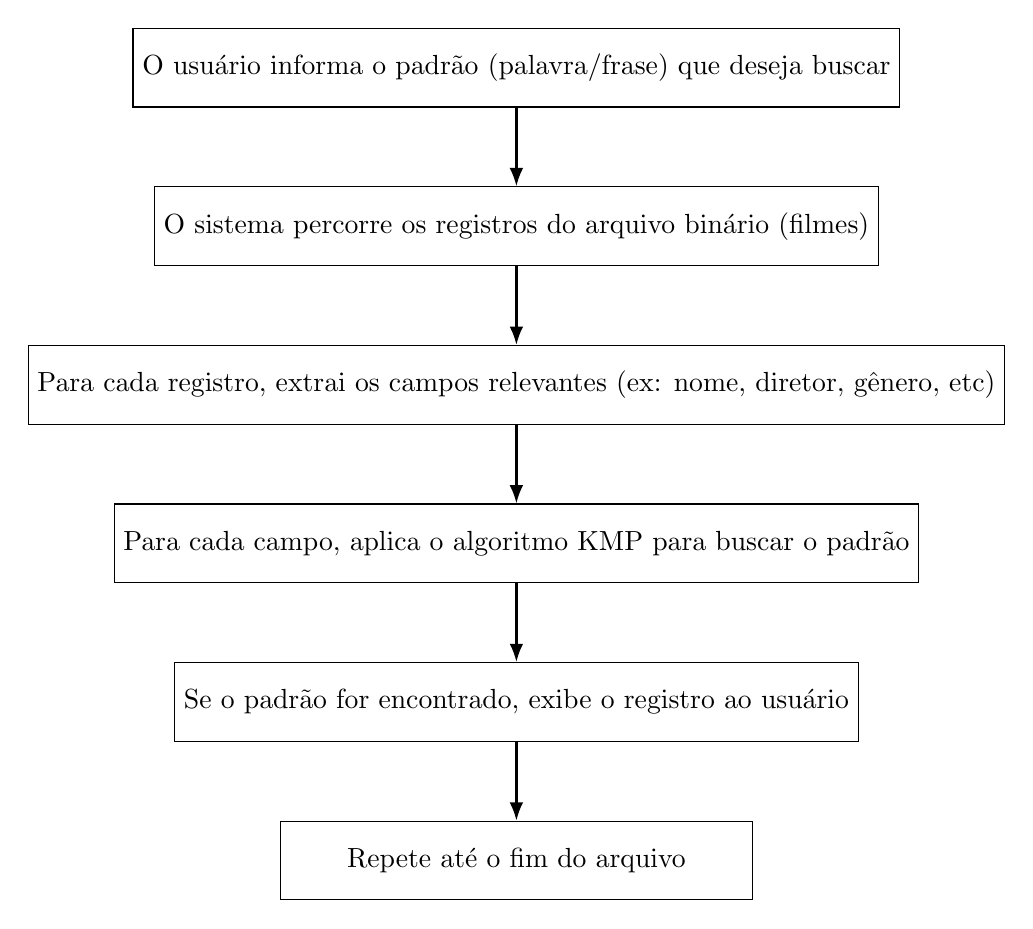
\begin{tikzpicture}[ 
node distance=1cm, 
box/.style={draw, 
rectangle, 
minimum width=6cm, 
minimum height=1cm, 
align=center}, 
arrow/.style={-{Latex}, thick} 
]

\node[box] (step0) {O usuário informa o padrão (palavra/frase) que deseja buscar}; 
\node[box, below=of step0] (step1) {O sistema percorre os registros do arquivo binário (filmes)}; 
\node[box, below=of step1] (step2) {Para cada registro, extrai os campos relevantes (ex: nome, diretor, gênero, etc)}; 
\node[box, below=of step2] (step3) {Para cada campo, aplica o algoritmo KMP para buscar o padrão}; 
\node[box, below=of step3] (step4) {Se o padrão for encontrado, exibe o registro ao usuário}; 
\node[box, below=of step4] (step5) {Repete até o fim do arquivo};

\draw[arrow] (step0) -- (step1); 
\draw[arrow] (step1) -- (step2); 
\draw[arrow] (step2) -- (step3); 
\draw[arrow] (step3) -- (step4); 
\draw[arrow] (step4) -- (step5);

\end{tikzpicture} 
\end{center}

\section*{Fluxo de Processamento de Conteúdo - Pré-processamento (KMP)} 
\begin{center} 
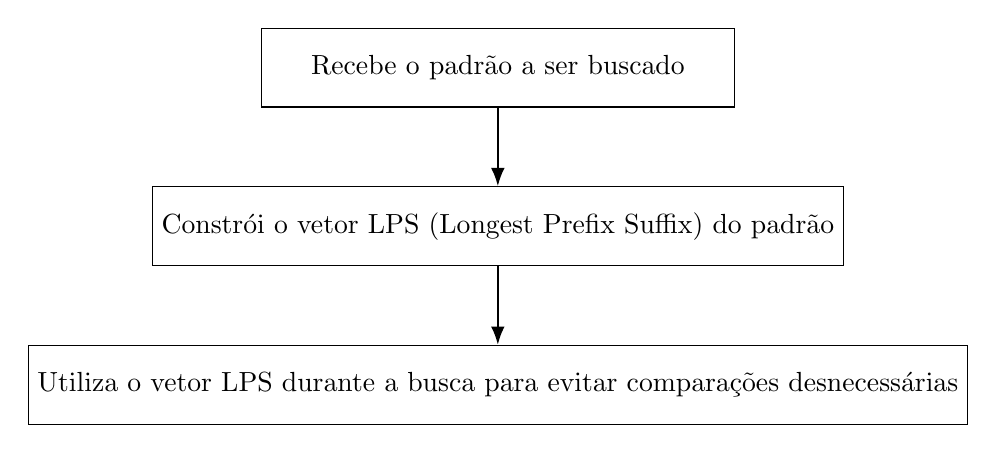
\begin{tikzpicture}[ 
node distance=1cm, 
box/.style={draw, 
rectangle, 
minimum width=6cm, 
minimum height=1cm, 
align=center}, 
arrow/.style={-{Latex}, thick} 
]

\node[box] (step0) {Recebe o padrão a ser buscado}; 
\node[box, below=of step0] (step1) {Constrói o vetor LPS (Longest Prefix Suffix) do padrão}; 
\node[box, below=of step1] (step2) {Utiliza o vetor LPS durante a busca para evitar comparações desnecessárias};

\draw[arrow] (step0) -- (step1); 
\draw[arrow] (step1) -- (step2);

\end{tikzpicture} 
\end{center}

\subsubsection{Resultados}
Com isso se conclui que a implementação de compressão e um fator importante quando se trata de grandes dados visto que em nosso código, que por mais que seja pequeno teve em media uma redução de 30\%. Com isso a busca de padrões e uma boa implementação, pois consegue identificar com precisão dados que tenham semelhanças com palavras nas quias você tenha interseção

\subsection{TP4}

Nesta ultima etapa teremos que implementar dois tipos de criptografia, uma Simples, podendo ser Substituição, Vigenére ou Transposição, e uma Moderna, sendo DES ou RSA.
Nos Decidimos por optar pela de Vigenére e pela DES, devido ao fato serem a que a que mais compreendemos e conseguimos resolver facilmente tanto a criptografia quanto a descriptografia.

\vspace{-4cm}

\subsubsection{Vigenére}
O principal diferencial do algoritmo de Vigenère é sua capacidade de proteger os dados por meio de criptografia simétrica, utilizando uma chave fornecida pelo usuário para embaralhar os bytes do arquivo. Isso garante confidencialidade e segurança das informações armazenadas e transmitidas no sistema, dificultando o acesso não autorizado.

A implementação do algoritmo de Vigenère, apesar de conceitualmente simples, exige atenção ao correto tratamento dos bytes e à aplicação da chave ao longo de todo o conteúdo. Em nosso projeto, estruturamos o processo da seguinte forma: durante a criptografia, o sistema solicita ao usuário uma chave, que é convertida em um vetor de bytes. Em seguida, cada byte do arquivo original é somado ao byte correspondente da chave (de forma cíclica), gerando um novo arquivo criptografado.

No momento da gravação, tanto os metadados quanto os dados dos registros são criptografados utilizando a chave informada, garantindo que todo o conteúdo do arquivo permaneça protegido. O processo é realizado de maneira transparente, sem alterar a estrutura dos dados, apenas modificando seus valores para impedir a leitura direta.

Na operação de descriptografia, o sistema solicita novamente a chave ao usuário. Utilizando o mesmo algoritmo, porém invertendo a operação, cada byte do arquivo criptografado é subtraído do byte correspondente da chave, restaurando assim o conteúdo original. Caso a chave informada esteja incorreta, os dados recuperados serão inválidos, protegendo a integridade das informações.

Por fim, a integração do algoritmo de Vigenère ao sistema foi feita de modo a permitir que a criptografia e descriptografia dos arquivos ocorram de forma simples e acessível, bastando ao usuário informar a chave desejada. Isso proporciona uma camada adicional de segurança no gerenciamento dos arquivos do projeto, sem comprometer a usabilidade ou a eficiência das operações.

\section*{Fluxo de Processamento de Conteúdo - Criptografia (Vigenère)} 
\begin{center} 
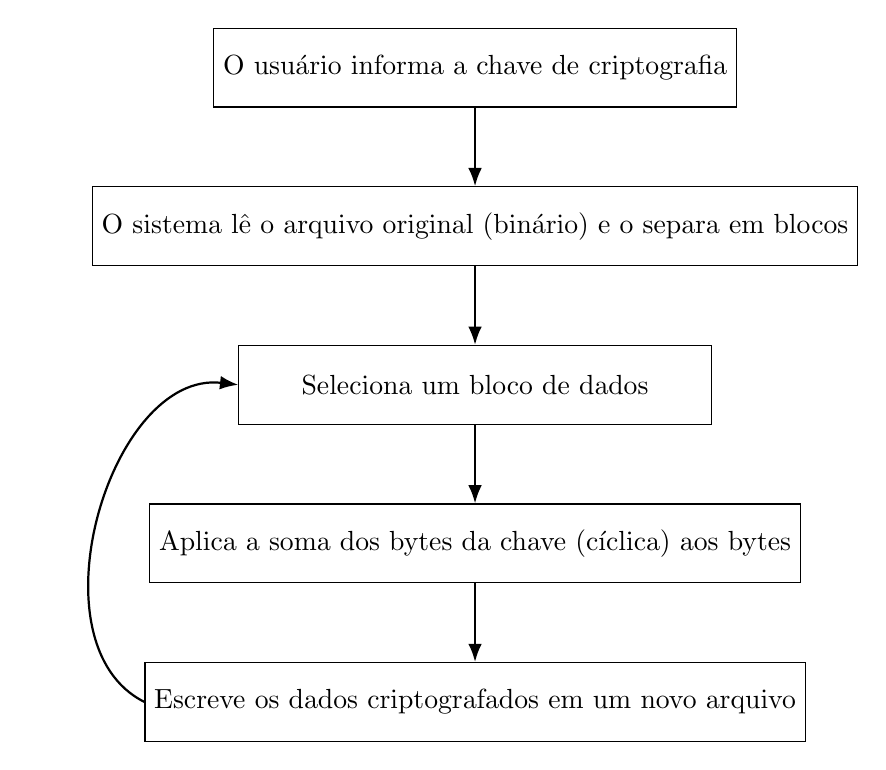
\begin{tikzpicture}[ 
node distance=1cm, 
box/.style={draw, 
rectangle, 
minimum width=6cm, 
minimum height=1cm, 
align=center}, 
arrow/.style={-{Latex}, thick} 
]

\node[box] (step0) {O usuário informa a chave de criptografia}; 
\node[box, below=of step0] (step1) {O sistema lê o arquivo original (binário) e o separa em blocos};
\node[box, below=of step1] (step2) {Seleciona um bloco de dados};
\node[box, below=of step2] (step3) {Aplica a soma dos bytes da chave (cíclica) aos bytes}; 
\node[box, below=of step3] (step4) {Escreve os dados criptografados em um novo arquivo}; 

\draw[arrow] (step0) -- (step1); 
\draw[arrow] (step1) -- (step2); 
\draw[arrow] (step2) -- (step3);
\draw[arrow] (step3) -- (step4);

\draw[arrow, bend left=80] (step4.west) to (step2.west);

\end{tikzpicture} 
\end{center}

\section*{Fluxo de Processamento de Conteúdo - Descriptografia (Vigenère)} 
\begin{center} 
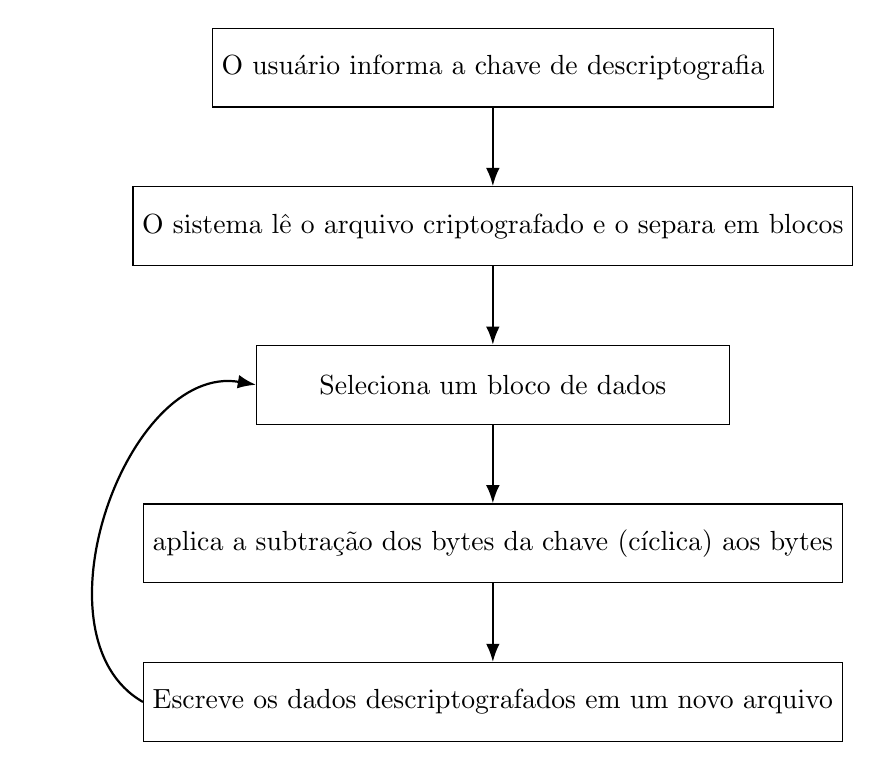
\begin{tikzpicture}[ 
node distance=1cm, 
box/.style={draw, 
rectangle, 
minimum width=6cm, 
minimum height=1cm, 
align=center}, 
arrow/.style={-{Latex}, thick} 
]

\node[box] (step0) {O usuário informa a chave de descriptografia}; 
\node[box, below=of step0] (step1) {O sistema lê o arquivo criptografado e o separa em blocos}; 
\node[box, below=of step1] (step2) {Seleciona um bloco de dados};
\node[box, below=of step2] (step3) {aplica a subtração dos bytes da chave (cíclica) aos bytes}; 
\node[box, below=of step3] (step4) {Escreve os dados descriptografados em um novo arquivo}; 

\draw[arrow] (step0) -- (step1); 
\draw[arrow] (step1) -- (step2); 
\draw[arrow] (step2) -- (step3);
\draw[arrow] (step3) -- (step4);

\draw[arrow, bend left=80] (step4.west) to (step2.west);

\end{tikzpicture} 
\end{center}

\subsubsection{DES}
O algoritimo de DES tem como seu lado forte sua capacidade de proteger os dados por meio de criptografia simétrica em blocos, utilizando uma chave secreta para embaralhar as informações de forma robusta. Isso garante a confidencialidade dos arquivos armazenados e transmitidos no sistema, dificultando o acesso não autorizado aos dados sensíveis.

A implementação do algoritmo DES, apesar de baseada em operações matemáticas bem definidas, exige atenção a detalhes como o gerenciamento dos blocos de dados, o uso correto das permutações e substituições, além do tratamento adequado do preenchimento (padding) dos dados. Em nosso projeto, estruturamos o processo da seguinte forma: durante a criptografia, o sistema solicita ao usuário uma senha, que é convertida em uma chave de 64 bits por meio de um hash. Os dados do arquivo são então divididos em blocos de 8 bytes, e cada bloco é criptografado individualmente utilizando a chave gerada.

No momento da gravação, tanto os metadados quanto os dados dos registros são criptografados em blocos, garantindo que todo o conteúdo do arquivo permaneça protegido. O processo é realizado de maneira transparente, sem alterar a estrutura dos dados, apenas modificando seus valores para impedir a leitura direta.

Na operação de descriptografia, o sistema solicita novamente a senha ao usuário. Utilizando a mesma chave, cada bloco criptografado é processado pelo algoritmo DES em modo reverso, restaurando assim o conteúdo original. O sistema também remove o preenchimento extra adicionado durante a criptografia, garantindo que os dados recuperados estejam íntegros. Caso a senha informada esteja incorreta, os dados descriptografados serão inválidos, protegendo a integridade das informações.

Por fim, a integração do algoritmo DES ao sistema foi feita de modo a permitir que a criptografia e descriptografia dos arquivos ocorram de forma simples e segura, bastando ao usuário informar a senha desejada. Isso proporciona uma camada adicional de segurança no gerenciamento dos arquivos do projeto, sem comprometer a usabilidade ou a eficiência das operações.

\section*{Fluxo de Processamento de Conteúdo - Criptografia (DES)} 
\begin{center} 
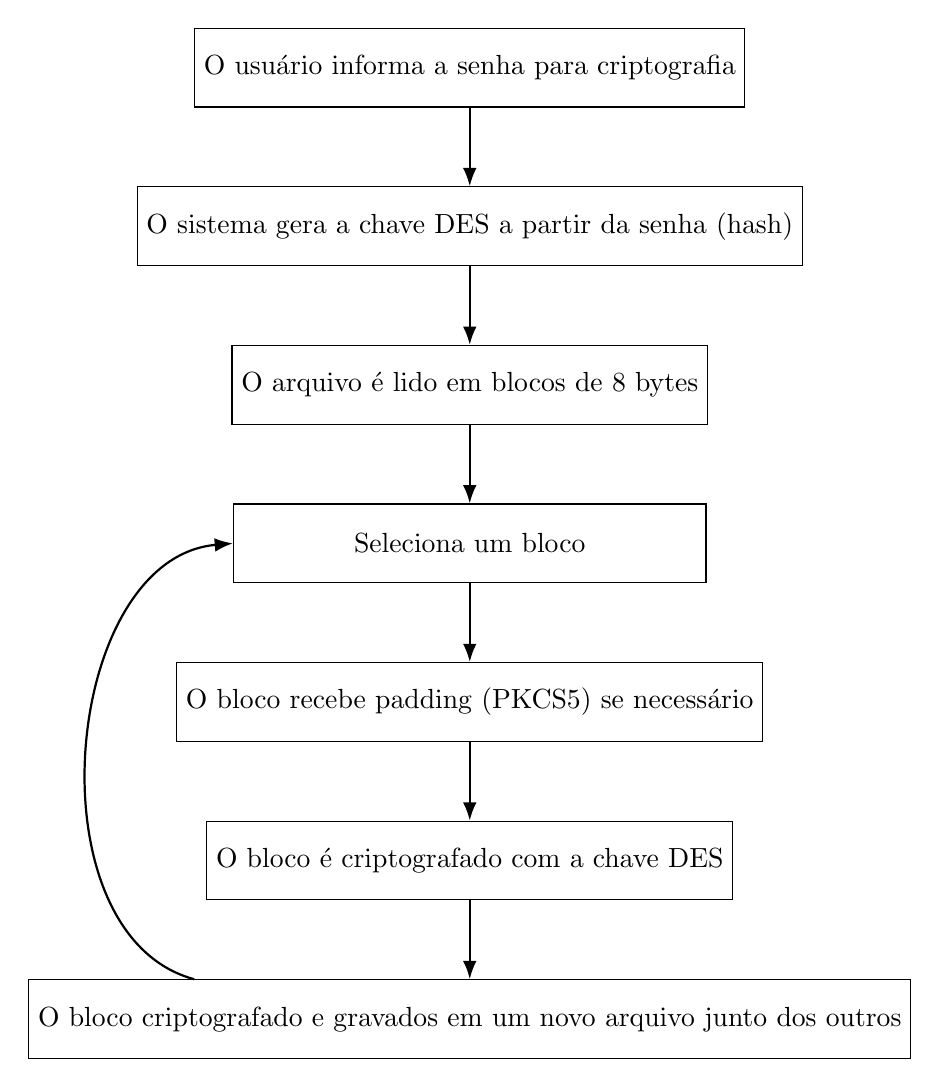
\begin{tikzpicture}[ 
node distance=1cm, 
box/.style={draw, 
rectangle, 
minimum width=6cm, 
minimum height=1cm, 
align=center}, 
arrow/.style={-{Latex}, thick} 
]

\node[box] (step0) {O usuário informa a senha para criptografia}; 
\node[box, below=of step0] (step1) {O sistema gera a chave DES a partir da senha (hash)}; 
\node[box, below=of step1] (step2) {O arquivo é lido em blocos de 8 bytes}; 
\node[box, below=of step2] (step3) {Seleciona um bloco};
\node[box, below=of step3] (step4) {O bloco recebe padding (PKCS5) se necessário}; 
\node[box, below=of step4] (step5) {O bloco é criptografado com a chave DES}; 
\node[box, below=of step5] (step6) {O bloco criptografado e gravados em um novo arquivo junto dos outros}; 


\draw[arrow] (step0) -- (step1); 
\draw[arrow] (step1) -- (step2); 
\draw[arrow] (step2) -- (step3); 
\draw[arrow] (step3) -- (step4); 
\draw[arrow] (step4) -- (step5); 
\draw[arrow] (step5) -- (step6);

\draw[arrow, bend left=80] ([xshift=-3.5cm]step6.north) to (step3.west);

\end{tikzpicture} \end{center}

\section*{Fluxo de Processamento de Conteúdo - Descriptografia (DES)} 
\begin{center} 
\begin{tikzpicture}[ 
node distance=1cm, 
box/.style={draw, 
rectangle, 
minimum width=6cm, 
minimum height=1cm, 
align=center},
arrow/.style={-{Latex}, thick} 
]

\node[box] (step0) {O usuário informa a senha para descriptografia}; 
\node[box, below=of step0] (step1) {O sistema gera a chave DES a partir da senha (hash)}; 
\node[box, below=of step1] (step2) {O arquivo criptografado é lido em blocos de 8 bytes};
\node[box, below=of step3] (step3) {Seleciona um bloco};
\node[box, below=of step3] (step4) {O bloco é descriptografado com a chave DES}; 
\node[box, below=of step4] (step5) {O padding é removido dos dados descriptografados}; 
\node[box, below=of step5] (step6) {Os dados originais são gravados em um novo arquivo}; 

\draw[arrow] (step0) -- (step1); 
\draw[arrow] (step1) -- (step2); 
\draw[arrow] (step2) -- (step3); 
\draw[arrow] (step3) -- (step4); 
\draw[arrow] (step4) -- (step5); 
\draw[arrow] (step5) -- (step6);

\draw[arrow, bend left=80] ([xshift=-3.5cm]step6.north) to (step3.west);

\end{tikzpicture} 
\end{center}

\subsection*{Resultado}
Por fim se conclui que as criptografias implementadas por mais que no mundo de hoje não sejam mais seguras, devido ao métodos de descriptografia avançados e ao avanço da computação se consegue quebrá-las em instantes, elas ainda servem para um proposito, que e a compreensão básico de como um criptografia funciona e como e implementada

\section{Conclusão}

Em suma, conclui-se que o projeto passou por diversos desafios ao longo de seu desenvolvimento, dando ênfase principalmente para o TP 2 por seu tamanho e nível de complexidade. Entretanto, a dupla obteve êxito e conseguiu realizar os códigos e suas devidas necessidades a tempo e de forma bastante clara e completa. 

\end{document}
